\documentclass{article}
\usepackage{iclr2027_conference,times}
\usepackage{amsmath,amssymb,amsthm,mathtools,booktabs,graphicx,microtype,xcolor}
\usepackage[hidelinks]{hyperref}
% Standard anonymous submission layout from the supplied ICLR 2027 template.
\newtheorem{theorem}{Theorem}
\newtheorem{proposition}[theorem]{Proposition}
\newtheorem{corollary}[theorem]{Corollary}
\newtheorem{lemma}[theorem]{Lemma}
\theoremstyle{remark}\newtheorem{remark}[theorem]{Remark}
\newcommand{\R}{\mathcal R}
\newcommand{\Rs}{\R_{\mathrm{stat}}^*}
\newcommand{\Rt}{\R_{2}^*}
\newcommand{\Ra}{\R_{\mathrm{all}}^*}
\newcommand{\Rp}{\R_{\mathrm{prep}}}
\newcommand{\tr}{\operatorname{tr}}
\newcommand{\op}{\mathrm{op}}
\newcommand{\E}{\mathbb E}
\newcommand{\norm}[1]{\left\lVert#1\right\rVert}
\newcommand{\eps}{\varepsilon}
\title{When Does Training Order Buy Compute?\\An Exact Curriculum--Mixture Boundary}
\author{Anonymous authors}
\date{}
\begin{document}
\maketitle
\begin{abstract}
A training curriculum can beat a chosen data mixture without beating the best fixed mixture. We study this stronger comparison in shared-optimum quadratic learning with a fixed optimizer. For two symmetric sources, we identify exactly when changing their weights over time can help. If the sources are separated by angle $\phi$ and the initial error has orthogonal second-moment mass $\varepsilon$, balanced mixing is globally optimal over all measurable schedules at budget $B$ if and only if $\varepsilon\ge e^{-2B\cos\phi}$. Below this boundary, two mixed phases suffice for a strict improvement. Just below it, the optimal relative gain is quadratic in the distance to the boundary, with sharp coefficient $1/8$. The proof combines a monotone indefinite quadratic form with a determinant constraint, and applies to any number of switches. We also construct a globally rate-optimal curriculum for a known error direction, separate loss improvements from compute savings, and give conditions under which shared curricula cannot change a power-law exponent. An additive-noise extension and exact Gaussian SGD calculations clarify the limits of the deterministic result. CPU experiments verify the boundary and show that improvements in stochastic training depend strongly on batch size, source sampling, and directional uncertainty. The result is a precise model-level account of when training order is useful, not a universal curriculum prescription.
\end{abstract}

\section{Introduction}
Training on several data sources requires two decisions: how much of each source to use, and when to use it. Scaling laws address allocations among model size, data, and training duration \citep{kaplan2020,hoffmann2022}; data-mixture methods also optimize source proportions \citep{ye2025,shukor2025,dai2026}. A curriculum adds the freedom to change those proportions as training proceeds. This freedom creates an appealing possibility: a source that is useful early may prepare the model to learn more efficiently from another source later. But it also creates a harder comparison problem. An ordering can outperform uniform sampling simply because uniform sampling uses the wrong proportions.

To establish a value for \emph{order itself}, the reference must therefore be the best fixed mixture at the same budget. Even matching the curriculum's total source exposure is not enough: another constant allocation could be better than both methods. Nor does a preference for $A$ followed by $B$ over the reverse order settle the question. Both orders may lose to mixing throughout training. We ask the stronger question: \emph{when can changing source weights beat every static mixture, and how much compute can that freedom save?} The static competitor is reoptimized for every budget, rather than selected once and reused across scales.

This question is related to, but distinct from, learning a good curriculum in a particular application. Dynamic data mixing and optimal-control approaches already select useful training schedules \citep{chen2025,gu2025,mori2025,zhao2026}. Local geometric analyses can predict which source should come first \citep{sweeney2026}. Our objective is a comparison theorem: a condition under which \emph{no} admissible schedule can help, together with a construction that helps when the condition fails. Such a result identifies what a scheduler must know and which improvements a more elaborate planner cannot obtain.

We study a model that isolates training order from conflicting tasks and changing targets. Both sources have quadratic population losses with the same minimizer, and the optimizer is fixed. The sources differ only in the directions of error that they reduce. A first source can reshape the remaining error so that a second source removes it quickly. This preparation is useful when the residual lies in a favorable direction. However, a schedule that prepares that direction can leave more error in a perpendicular direction. Its value therefore depends not only on source geometry, but also on the \emph{initial second moment}: the average squared error in each direction across the training problems to which the same schedule is applied.

The main result makes this tradeoff exact. For two symmetric source directions separated by an acute angle $\phi$, let $\varepsilon$ be the initial error mass perpendicular to their bisector, normalized so that the bisector mass is one. At budget $B$, balanced static mixing is globally optimal over \emph{all measurable schedules} if and only if $\varepsilon\ge e^{-2B\cos\phi}$. The statement permits arbitrarily many costless switches. Below the boundary, two mixed phases already suffice for a strict benefit; above it, no additional scheduling complexity can help. The schedule is chosen before drawing the initial error. A policy that observes each realized residual and then selects its own schedule has more information and is not covered by this claim.

Two consequences change how the benefit should be interpreted. For every fixed positive orthogonal mass, static mixing becomes \emph{exactly optimal} after a finite budget. Thus a useful ordering may have a limited budget window, even with perfectly known source geometry. Moreover, a strict advantage is not necessarily a worthwhile one. Just below the boundary, the best relative improvement is quadratic in the distance to it, with coefficient $1/8$. Close to the threshold, estimating the geometry or searching for a schedule could cost more than the training benefit. Equal-budget loss ratios must also be distinguished from savings in work needed to reach a target loss.

Our theoretical contribution has three parts. We obtain an exact budget-optimal static benchmark and a necessary-and-sufficient comparison against arbitrary schedules. We then quantify the benefit through a matching near-boundary expansion and a globally rate-optimal construction for a known direction. Finally, we connect this finite-dimensional result to additive noise and shared block-spectral models, giving conditions under which scheduling cannot change a power-law exponent. The proof uses constraints on the entire training trajectory, rather than treating a local order effect as evidence of a global advantage.

The experiments follow the same separation of questions. Exact matrix calculations check the formulas. Exact expected Gaussian SGD tests whether useful schedules remain when gradients are noisy, using a bracket over \emph{all} static mixture weights. Finite-data and small nonlinear experiments test a direct transfer of the preparation rule, and retain its failures. Gains in the stochastic model depend on batch size and how sources are sampled within a batch; the nonlinear test is negative. The paper therefore offers a precise account of when order is valuable in a controlled model, not a universal recipe for neural-network training.

\section{Related work}
\paragraph{Curriculum learning.}
Curriculum learning has long studied useful presentation orders \citep{bengio2009}. Transfer-based and convex analyses connect example difficulty to convergence \citep{weinshall2018,weinshall2020}; empirical work shows that benefits depend on the training regime \citep{hacohen2019,wu2021}. Teacher--student analysis separates learning-speed benefits from changes in final performance \citep{saglietti2022}. Task-level curricula also study the order of distinct learning problems \citep{pentina2015}. We do not claim that curricula can help for the first time. Our comparator is the globally best static mixture within a stated dynamics, and our principal obstruction concerns directional initial-error mass.

\paragraph{Data-mixture optimization.}
DoReMi and DoGE learn useful domain weights through proxy optimization \citep{xie2023,fan2024}. Skill-it and Aioli exploit skill structure or update mixture parameters during training \citep{chen2023,chen2025}. RegMix predicts effective static mixtures, while RegMix-D explicitly transfers dynamic schedules from proxy trajectories \citep{liu2025,zhao2026}. Olmix studies mixture design and reuse as the domain set changes \citep{chen2026}. Mixture scaling laws predict losses across source proportions and scales \citep{ye2025,shukor2025}; \citet{dai2026} explain static mixing through capacity competition and noise reduction. Dynamic mixtures, proxy-based scheduling, and theoretical mixture models are therefore established ideas. Our results instead give an exact static benchmark, global schedule-rate comparisons, and a necessary-and-sufficient boundary over all measurable schedules in a deliberately controlled model.

\paragraph{Geometry and control.}
\citet{sweeney2026} uses Lie brackets to predict local transfer order. \citet{mori2025} derive task-selection protocols from exact learning dynamics and optimal control; \citet{gu2025} formulate language-model data selection using Pontryagin conditions. Switched linear systems also have an established control-theoretic treatment \citep{liberzon2003}. A control formulation, a commutator calculation, or a local numerical schedule search is not our contribution. Noncommutativity alone is insufficient for our stronger static-mixture comparison. We use the classical Golden--Thompson inequality \citep{golden1965,thompson1965} and scalar spectral Jensen inequalities explicitly, and do not present their corollaries as new matrix inequalities.

\paragraph{Spectral scaling.}
Solvable regression and random-feature models explain scaling through spectral tails and training dynamics \citep{maloney2022,bordelon2022,bordelon2024}. Feature learning can change that picture \citep{bordelon2025}. Our block result is a comparison statement: under a common spectral envelope and a uniformly adequate static mixture, a shared schedule cannot improve the exponent. It neither replaces those scaling theories nor covers feature learning in a general neural network. Finally, our perturbation and confidence calculations use standard matrix-exponential and Gaussian concentration tools \citep{higham2008,boucheron2013}; the decision being certified is the paid curriculum-versus-full-budget-static comparison.



\section{Model and the exact static comparator}\label{sec:model}
\subsection{What is held fixed, and what the scheduler controls}
Consider $L_i(\theta)=\tfrac12(\theta-\theta^*)^\top H_i(\theta-\theta^*)$ for $i\in\{A,B\}$, with $H_i\succeq0$ and a common target $\theta^*$. For example, these losses arise from realizable linear regression with source covariance $H_i$, after subtracting any irreducible label-noise loss. There is no disagreement about the correct predictor. Differences in training arise because a source provides more curvature, and hence faster error reduction under gradient flow, in some directions than in others.

If source $i$ costs $c_i>0$ per unit of gradient-flow time, define $G_i=H_i/c_i$. With normalized work $t$ and fraction $p(t)$ of the instantaneous work allocated to source $A$, the error follows
\begin{equation}
 \dot e(t)=-G(p(t))e(t),\qquad G(p)=pG_A+(1-p)G_B.\label{eq:dynamics}
\end{equation}
The scheduler changes only $p(t)$. It does not change the optimizer, learning-rate convention, model, or target. Work is the resource in this specified dynamics, not a hardware-independent count of floating-point operations. The normalization permits unequal source costs, but the exact theorem below requires the resulting \emph{normalized} generators to have the stated symmetry.

A schedule $\pi$ is a measurable function $p:[0,B]\to[0,1]$ chosen before drawing $e_0$. It may use the known source matrices and initial-error second moment, but not the realized error. For finite phases, its transition is
$\Phi_\pi=e^{-b_KG(p_K)}\cdots e^{-b_1G(p_1)}$, where $\sum_k b_k=B$; the rightmost phase acts first. Intermediate weights are allowed within each phase. Switching and planning are free in the main comparison. This favors curricula; the existence of a beneficial path need not survive a charge for finding or switching it.

Let $S=\E[e_0e_0^\top]$ and let $Q\succeq0$ weight errors at evaluation. The expected target loss is
\begin{equation}
 \R(\pi)=\tfrac12\tr(Q\Phi_\pi S\Phi_\pi^\top).\label{eq:risk}
\end{equation}
For linear prediction, $Q$ can be the target input covariance. The theorem uses $Q=I$, so it measures total squared parameter error. Write $\Rs,\Rt,\Ra$ for the infima over static mixtures, at most two phases, and all measurable schedules. Because a static weight is a valid curriculum, $\Ra\le\Rt\le\Rs$. A numerical candidate supplies an upper bound on optimal curriculum risk; it does not establish the optimum.

\subsection{A source family with interpretable error directions}
Take unit source directions $v_A=(1,0)^\top$ and $v_B=(\cos\phi,\sin\phi)^\top$, with $0<\phi<\pi/2$. Let $u$ be their unit bisector and $v$ its counterclockwise perpendicular. Set
\begin{equation}
 G_A=v_Av_A^\top+\rho I,\quad G_B=v_Bv_B^\top+\rho I,\quad
 S=uu^\top+\varepsilon vv^\top,\quad Q=I,\qquad \rho,\varepsilon\ge0.\label{eq:mainfamily}
\end{equation}
The shared ridge $\rho$ gives both sources some curvature in every direction. Without it, each source teaches only one direction, while an interior mixture still learns both. These are Gaussian source covariances for one shared linear regression target, not two tasks with incompatible labels.

The parameter $\varepsilon$ describes residual variation, not measurement error in the source matrices. One concrete ensemble is $e_0=u+\sqrt\varepsilon\,Z v$, where $\Pr(Z=1)=\Pr(Z=-1)=1/2$. Its mean is $u$, its covariance is $\varepsilon vv^\top$, and its \emph{second moment} is exactly $S$. At $\varepsilon=0$ the error direction is known. At $\varepsilon=1$ the second moment is isotropic, even though the mean need not vanish. The ensemble is held fixed while $B$ changes; $\varepsilon$ is not a posterior confidence radius that training automatically updates.

Put $c=\cos\phi$, $a=(1+c)/2$, and $d=(1-c)/2$. In the $(u,v)$ basis,
\begin{equation}
 G(p)=\begin{pmatrix}\rho+a&z\\z&\rho+d\end{pmatrix},\qquad
 z=(1-2p)\sqrt{ad}.\label{eq:mirror}
\end{equation}
Balanced mixing has $z=0$. It reduces the bisector error at rate $\rho+a$ and the perpendicular error at the slower rate $\rho+d$. Other weights couple the two directions without changing those diagonal entries. This separation makes it possible to study preparation against an exactly optimized static reference.

\subsection{The benchmark and the meaning of a gain}
\begin{proposition}[Exact best static mixture]\label{main:static}
For every $B\ge0$ and $\varepsilon\ge0$, balanced mixing $p=1/2$ globally minimizes static risk, with
\begin{equation}
 \boxed{\Rs(B,\varepsilon)=\tfrac12\left[e^{-2(\rho+a)B}+\varepsilon e^{-2(\rho+d)B}\right].}\label{eq:mainstatic}
\end{equation}
\end{proposition}
\emph{Reason.} Every mixture has the same diagonal in this basis. Scalar Jensen applied to a vector's spectral measure gives $u^\top e^{-2BG}u\ge e^{-2B u^\top Gu}$, and likewise for $v$. Balanced mixing attains both bounds. Appendix~\ref{app:exact} gives the common-diagonal statement. This is an application of a classical inequality, not a new matrix inequality. Crucially, the comparator is optimized over every constant weight, not chosen for convenience.

We report gain as static risk divided by curriculum risk, so one means a tie and values below one mean that a candidate is worse. Optimal gain is at least one because doing no scheduling is allowed. This alone is not evidence of a useful method. A meaningful empirical gain must exceed numerical uncertainty and, for a practical allocator, pay for obtaining the schedule. Section~\ref{sec:consequences} separately compares the work required to reach a common loss target; that work ratio need not equal an equal-budget loss ratio.

\section{Exactly when any curriculum can help}\label{sec:boundary}
\begin{theorem}[Global curriculum--mixture boundary]\label{main:boundary}
For \eqref{eq:mainfamily} and $B>0$, balanced static mixing is optimal over all measurable schedules if and only if
\begin{equation}
 \boxed{\varepsilon\ge\varepsilon_{\rm crit}(B):=e^{-2B\cos\phi}.}\label{eq:mainboundary}
\end{equation}
Below this boundary, a schedule with two mixed phases strictly improves on every static mixture. In particular, for $0<\varepsilon<1$,
\begin{equation}
 B\ge B_{\rm stop}(\varepsilon):=\frac{\log(1/\varepsilon)}{2\cos\phi}
 \quad\Longrightarrow\quad\Ra(B,\varepsilon)=\Rt(B,\varepsilon)=\Rs(B,\varepsilon).
\end{equation}
\end{theorem}
The result does not restrict the number of switches or impose a switching cost. This makes the no-benefit side stronger. On the other side it proves existence of a useful two-phase schedule, not an exact formula for the globally best schedule below the boundary. For $\phi=45^\circ$ and $\varepsilon=0.01$, the stopping boundary is $B\approx3.256$: beyond that budget, even unlimited costless switching cannot improve the population risk.

\subsection{Why the no-benefit side is global}
The proof uses two facts about the entire transition, rather than comparing adjacent phases. Start the dynamics at $v$, and write its coordinates as $(x(t),y(t))$. The off-diagonal control cancels from the derivative of $W=y^2-x^2$:
\begin{equation}
 W'=-2(\rho+d)W+2c x^2,\qquad W(0)=1.
\end{equation}
Hence $\|\Phi v\|^2\ge e^{-2(\rho+d)B}$. In plain language, switching cannot reduce the error from the slow initial direction faster than balanced mixing does. This does not prevent it from accelerating the other direction.

Now let $f=\Phi u$, $g=\Phi v$, $t=\|g\|^2$, and $k=f^\top g$. Every generator has trace $1+2\rho$, so the squared determinant is $D=e^{-2(1+2\rho)B}$. The Gram determinant identity gives
\begin{equation}
 2\R(\pi)=\frac{D+k^2}{t}+\varepsilon t
 \ge\frac{D}{t}+\varepsilon t,\qquad t\ge b:=e^{-2(\rho+d)B}.\label{eq:maingram}
\end{equation}
When $\varepsilon\ge D/b^2=e^{-2cB}$, the right side is nondecreasing for $t\ge b$. Balanced mixing attains its minimum at $t=b,k=0$. The quadratic-form bound and determinant therefore rule out \emph{every} schedule, including infinitely many switches. Appendix~\ref{app:global} treats bounded measurable controls directly.

\subsection{Why two phases suffice below the boundary}
To prove the other direction, perturb balanced mixing rather than guessing a pure-source order. Let the off-diagonal entry be $\eta q$ in the first half of training and $-\eta$ in the second, where
\begin{equation}
 q=\frac1{2\cosh(cB/2)-1},\qquad 0<\eta\le\sqrt{ad}.\label{eq:mainwitness}
\end{equation}
This choice cancels the first-order change in the column inner product $k$. The slow column length increases as $t=b+K\eta^2+O(\eta^4)$ for an explicit $K>0$, while $k=O(\eta^3)$. Substitution into the exact identity \eqref{eq:maingram} gives
\begin{equation}
 \R(\pi_\eta)-\Rs=\tfrac K2(\varepsilon-e^{-2cB})\eta^2+O(\eta^4).
\end{equation}
Below the boundary the leading term is negative. A sufficiently small perturbation therefore beats the globally optimized static baseline. The proof also holds for mirror sources with arbitrary diagonals $a_0>d_0>0$ and off-diagonal range $[-h,h]$, $0<h\le\sqrt{a_0d_0}$; their boundary is $e^{-2(a_0-d_0)B}$.

\begin{figure}[t]
\centering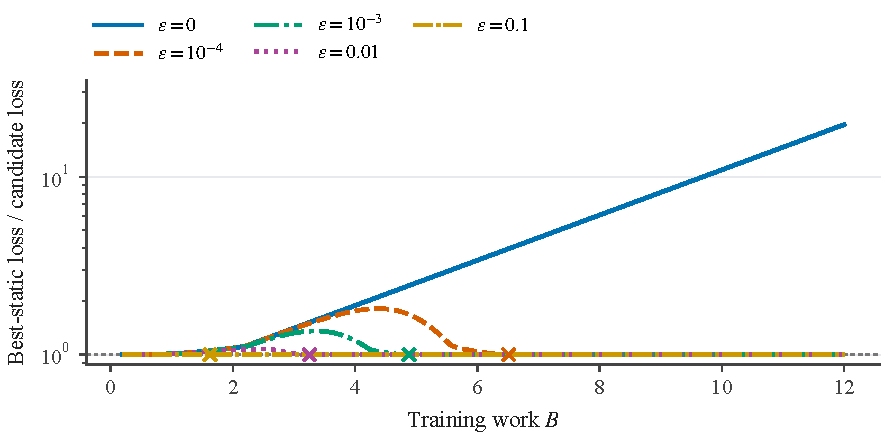
\includegraphics[width=.92\linewidth]{figures/global_boundary.pdf}
\caption{A useful curriculum can have a finite budget window. At $45^\circ$, plotted curves are attainable candidate gains, not claimed optima below the boundary. Crosses mark the exact stopping budgets: the best possible gain is one thereafter. The initial-error mass $\varepsilon$ is varied while source geometry is fixed.}\label{fig:global}
\end{figure}

\subsection{A strict benefit can still be too small to matter}
The Gram lower bound is also quantitatively sharp near the boundary.
\begin{theorem}[Sharp near-boundary gain]\label{main:near}
Fix $B>0$, $\phi$, and $\rho$. For $\varepsilon=e^{-2cB}(1-\xi)$ and $\xi\downarrow0$,
\begin{equation}
 \boxed{\frac{\Rs}{\Rt}-1=\frac{\xi^2}{8}+O(\xi^3),\qquad
 \frac{\Rs}{\Ra}-1=\frac{\xi^2}{8}+O(\xi^3).}\label{eq:mainnear}
\end{equation}
\end{theorem}
The lower envelope from \eqref{eq:maingram} is $\sqrt\varepsilon e^{-(1+2\rho)B}$. A perturbation in \eqref{eq:mainwitness} with $\eta^2=b\xi/(2K)$ attains it to error $O(\xi^3)$; a Taylor expansion proves the result (Appendix~\ref{app:near_boundary}). The constants are not uniform as the budget or source off-diagonal strength tends to zero. At relative boundary distance $\xi=0.1$, the leading gain is only $0.00125$, or $0.125\%$. Thus the exact boundary should not be interpreted as a recommendation to spend resources whenever strict improvement is possible.

\section{Compute savings, noise, and scaling}\label{sec:consequences}
\paragraph{A known direction can benefit substantially.}
At $\varepsilon=0$, a simple pure-source curriculum first trains on $A$ for $\tau=\log((1+c)/c)$, which aligns the residual with $v_B$, then trains on $B$. For $B\ge\tau$, its exact loss is $A_\phi e^{-2(1+\rho)B}/2$, where $A_\phi=a/c^2$. No schedule can contract any vector faster than rate $1+\rho$, so
\begin{equation}
 \tfrac12e^{-2(1+\rho)B}\le\Ra(B,0)\le\Rt(B,0)\le\tfrac{A_\phi}{2}e^{-2(1+\rho)B}.
\end{equation}
The construction is globally rate-optimal up to a budget-independent factor, not exactly optimal at every budget. Its static-to-curriculum loss ratio grows as $A_\phi^{-1}e^{2dB}$. In contrast, the ratio of work needed to attain the same small target loss tends to $(\rho+1)/(\rho+a)<2$. At $45^\circ$ and zero ridge, the loss gains are $1.8904$ at $B=4$ and $6.1003$ at $B=8$, but the limiting work ratio is only $1.1716$. Appendix~\ref{app:exact} proves these formulas and Appendix~\ref{app:uncertainty} treats uncertainty for this particular rule.

\paragraph{Noise puts a further limit on gains.}
Consider the separate additive-noise model $de=-G(p(t))e\,dt+\sigma\,dW$ with a deterministic schedule. Every schedule pays at least the balanced mixture's noise contribution
\begin{equation}
 N(B)=\frac{\sigma^2}{4}\left[\frac{1-e^{-2(\rho+a)B}}{\rho+a}+\frac{1-e^{-2(\rho+d)B}}{\rho+d}\right].\label{eq:mainnoise}
\end{equation}
Indeed, each injected isotropic error propagates through an admissible suffix schedule; Theorem~\ref{main:boundary} with $\varepsilon=1$ applies to each suffix. Adding the deterministic lower envelope proves that static mixing is still optimal above the same \emph{sufficient} boundary. For any fixed $\sigma>0$, the best possible gain tends to one as $B$ grows, even at $\varepsilon=0$ (Appendix~\ref{app:diffusion}). The deterministic boundary is not asserted necessary under noise, and SGD is not assumed to equal this diffusion.

\paragraph{Order need not change a scaling exponent.}
To connect finite-dimensional dynamics with power laws, consider blocks with scales $\lambda_j\asymp j^{-\alpha}$ and initial masses $w_j\asymp j^{-1-\beta}$. All blocks must share \emph{one} schedule. Suppose $0\preceq G_{i,j}\preceq L\lambda_j I$ and one static mixture obeys $G(p_0)_j\succeq m\lambda_j I$, uniformly in $j$. For $B\ge1$ and capacity $J\ge1$, including the entire untrained tail, both the best shared schedule and this static mixture attain
\begin{equation}
 \R^*(B,J)\asymp B^{-\beta/\alpha}+J^{-\beta}.
 \qquad \inf_{JB\le C}\R^*(B,J)\asymp C^{-\beta/(\alpha+1)}.\label{eq:mainscaling}
\end{equation}
Capacity is chosen before training; $C=JB$ is the assumed model-work accounting. A block cannot contract faster than its upper rate bound, and the static mixture attains a comparable rate in every block. A tail-sum bound and capacity--duration balance give \eqref{eq:mainscaling}. Theorem~\ref{thm:spectral} and Appendix~\ref{app:spectral} give the precise statement and proof. These assumptions rule out exponent changes, not all constant-factor gains, and need not hold for feature-learning networks.

\section{Experiments: strong comparators and mixed outcomes}\label{sec:experiments}
The experiments ask three different questions: do independent computations reproduce the theoretical boundary; does useful scheduling survive stochastic gradients; and does the preparation rule transfer when its assumptions fail? All experiments are CPU-only and synthetic. Exact-model checks support implementation correctness, not an empirical claim about large models. Complete grids, seeds, and failure cases appear in Appendices~\ref{app:extension_experiments} and \ref{app:experiments}.

\subsection{Checking the boundary rather than only finding favorable examples}
Across 1,200 random schedules with 1 to 64 phases, we observe no violation of the global lower bound. The audit varies source angle, ridge, budget, and initial mass on both sides of the boundary; it includes pure and mixed phases. Independently, 150 matrix-exponential calculations at 80-digit precision verify the predicted signs of the two-phase perturbation. High precision matters here because the difference from balanced mixing can be much smaller than either loss. Forty-five near-boundary checks recover the coefficient $1/8$, while 480 random diffusion schedules satisfy both noise and total-risk lower bounds.

Figure~\ref{fig:global} shows attainable gains from a small candidate family, not a numerical estimate of the global optimum below the boundary. The marked stopping budgets are exact: after each crossing, balanced mixing is optimal over the entire schedule class. Above the threshold, failure of a numerical search is therefore not the reason we conclude that scheduling cannot help. Conversely, below it, our proof establishes a strict advantage even when a finite candidate search cannot resolve a very small one. The high-precision checks and near-boundary plot in Appendix~\ref{app:extension_experiments} separate these cases.

\subsection{Exact expected SGD with two source-sampling conventions}
We next use fresh Gaussian linear-regression examples with a common target and independent label noise. For a pure source with covariance $H$, batch size $m$, and step $\eta$, Gaussian fourth moments give the exact update of $S=\E[ee^\top]$:
\begin{equation}
 S^+=S-\eta(HS+SH)+\eta^2\left[(1+m^{-1})HSH+m^{-1}\tr(HS)H\right]
 +\eta^2\sigma_y^2H/m.
\end{equation}
Composing these moment updates gives expected terminal risk directly, without fitting a learning curve or estimating it from a finite set of training seeds. Appendix~\ref{app:moments} derives the closure, including the fourth moments of mixed batches. The pure-source formula should not simply be applied to the average covariance of a non-Gaussian mixture.

Our primary convention samples a domain independently for \emph{each example}. The secondary convention chooses one domain for the \emph{entire minibatch}. Both have the same expected gradient at a given parameter, but not the same gradient fluctuations. Averaging a per-example batch can reduce variability in its source composition; choosing a single source for the whole batch retains that component of noise. The conventions agree for batch size one and for pure sources. Distinguishing them prevents a change in sampling noise from being mistaken for a deterministic ordering effect.

The condition grid uses angles $30^\circ,45^\circ,65^\circ$; $B\in\{1,4,8\}$; steps $\eta\in\{0.01,0.05\}$; batches $m\in\{1,8,64\}$; label standard deviations $0,0.1$; and $\varepsilon\in\{0,10^{-4},0.01,0.1\}$, with ridge $0.02$. Each convention has 432 conditions. Within a comparison, all methods use the same $K=B/\eta$ updates and $Km$ examples. Across different step or batch settings, the same $B$ does not imply the same example count or hardware cost. We compare source allocation within each training protocol, not joint optimization of batch size, learning rate, and schedule.

\paragraph{A comparator covering all static weights.}
For each condition, a curvature bound controls the risk between evaluated weights and supplies a global lower/upper bracket for the best static risk. No convexity assumption is imposed. All 864 brackets have relative width below $0.001$; these are float64 evaluations of an analytical bound, not directed-rounding certificates. A candidate must improve by over 1\% against the \emph{lower} bracket to enter the gain count. Reported median gains instead use the best evaluated static risk, the \emph{upper} bracket. Thus an unresolved gap between grid points cannot explain the counted advantage; the bracket width limits the approximation in the descriptive medians.

The candidate library includes every integer pure-source switch time in both orders, seven mixed perturbation amplitudes, and the best static grid point. It knows the population moments and its search cost is uncharged. The separately reported \emph{flow rule} is the unchanged preparation construction from Section~\ref{sec:consequences}, with its switch rounded to an update; it is feasible in 384 of 432 settings per convention. The library tests whether useful schedules exist under SGD noise, whereas the flow rule tests whether the simple deterministic prescription transfers. Neither is a globally optimized stochastic schedule.

\subsection{What the stochastic comparisons establish}
\begin{table}[t]
\centering\small
\caption{Exact expected SGD over the full condition grid. Median gains use the upper static bracket divided by candidate loss; $>1\%$ counts use the lower bracket. The oracle library includes static mixing; flow-rule medians use its 384 feasible conditions per convention.}\label{tab:mainmoments}
\begin{tabular}{lrrrr}\toprule
Source sampling & Cases & $>1\%$ gains & Median candidate gain & Median flow-rule gain\\\midrule
Per example &432&186&1.0033&0.7368\\
Per batch &432&220&1.0112&0.7910\\\bottomrule
\end{tabular}
\end{table}

Under per-example mixing, 186 of 432 conditions exceed a 1\% improvement against every static weight according to the lower bracket. The median candidate gain is only $1.0033$, and the unadapted flow rule has median $0.7368$. These counts describe a fixed grid of model configurations, not a success probability over an application population. Since the library includes the static option, ties are expected and nonnegative candidate gain alone is not evidence that arbitrary curricula are safe.

The sampling convention changes the magnitude of the apparent benefit. At batch size 64 and $B=4$, median candidate gain is $1.1633$ with per-example mixing and $1.5414$ with per-batch mixing. At $B=8$, the convention-wide medians are one. Figure~\ref{fig:sgdmoments} and the full table in Appendix~\ref{app:extension_experiments} retain the settings where gains disappear. This pattern is consistent with a limited useful budget window, but it does not establish that the deterministic boundary remains exact for SGD.

\begin{figure}[t]
\centering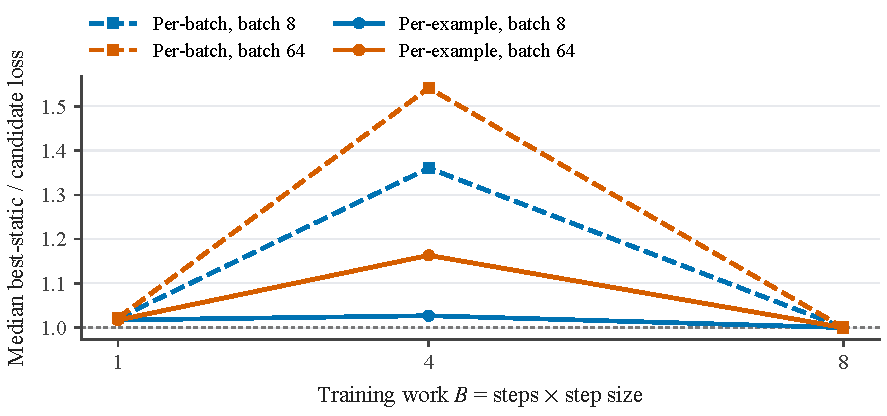
\includegraphics[width=.92\linewidth]{figures/sgd_moment_comparison.pdf}
\caption{Median oracle-library gains in exact Gaussian SGD, using the upper static bracket. Solid curves mix sources independently per example; dashed curves choose a source for the entire batch. Each point aggregates 48 conditions. Source-sampling noise changes the apparent benefit, even with identical population losses.}\label{fig:sgdmoments}
\end{figure}

As an independent implementation check, Monte Carlo training uses 8,192 trajectories per condition in 32 settings, covering both source conventions, static and two-phase methods, and two batch sizes. All sample means lie within three standard errors of the exact moment prediction; the largest absolute standardized discrepancy is $2.096$. This checks the moment implementation against actual sampled training. It is not a simultaneous confidence guarantee across all conditions. The main-grid risks themselves have no finite-trial sampling error, although numerical approximation and model misspecification remain separate issues.

\subsection{Paying for information and departing from the model}
The population comparisons assume known geometry. A separate confidence gate pays for noisy coordinate measurements of a residual and a declared planning cost. It accepts only when a candidate's upper risk bound beats a lower bound for a full-budget static competitor that did not buy the pilot (Appendix~\ref{app:certificate}). At positive planning charge, it accepts 23 of 2,160 trials, with no observed false acceptance. Median accepted gain is $1.400$, but median gain over \emph{all} outcomes is $0.403$. Rejecting a schedule does not refund the pilot. This supports a conditional acceptance certificate, not an overall policy of always buying measurements.

The finite-data and nonlinear tests address a different claim: whether the unchanged flow preparation rule is already a useful training prescription. Finite-data SGD gives 159 wins out of 320 paired comparisons and median gain $0.9944$. A width-16 tanh network trained in both layers gives 11 wins out of 48, with median gain $0.8980$. Their static weights are chosen in hindsight per seed, with tuning cost uncharged, rather than certified over all weights. These baselines are strong finite grids, but should not be confused with the exact static optimum in the theorem or the all-weight bracket in the moment experiment.

The nonlinear failure shows that input-source geometry alone does not justify this transferred schedule; it does not prove that no learned curriculum could work. Separately, a shared spectral schedule search finds maximum gain only $1.00314$, while capacity experiments recover the predicted exponents. Together the results support a narrow conclusion: the proved mechanism is real, but exploiting it under noisy gradients, uncertain geometry, or feature learning requires more than reusing the deterministic switch rule.

\section{Discussion and limitations}\label{sec:discussion}
The main theorem answers a global question exactly in a controlled model: when can changing data weights beat every fixed mixture? The answer depends not just on noncommuting source geometry, but on the remaining error in the other direction and the available budget. A monotone quadratic form limits what switching can do; a determinant constraint turns that limitation into an exact boundary. Two phases suffice to cross the boundary, and they attain the sharp leading gain near it.

Several boundaries of the result matter. Schedules are precommitted for an initial-error ensemble, not feedback policies that inspect each realized residual. The exact theorem uses mirror-source geometry and identity target risk; arbitrary Hessian perturbations, target anisotropy, and feature learning are not covered. The boundary says when a strict benefit exists, not whether it pays for switching, calibration, or search. The noisy result treats a stated isotropic diffusion, while SGD uses a separate exact moment model with fresh data. Candidate SGD schedules assume oracle moments and do not establish a budget-accounted learning algorithm. The spectral result assumes uniformly comparable block rates and a fixed adequate mixture.

The numerical experiments expose rather than resolve these practical limitations. Stochastic gains are conditional, the unadapted preparation rule often fails, and the nonlinear test is negative. The resulting contribution is a precise comparison theorem with testable quantitative consequences. It separates a genuine value of training order from the directional information and statistical conditions required to obtain it.
\label{main:end}

\clearpage
\section*{AI use statement}\label{sec:ai}
Generative AI was used substantially in this project, including proposing and developing proofs, writing and revising the manuscript, implementing and running synthetic experiments, generating figures, and assisting literature checks. The supplied tests and proof audits are part of this AI-assisted workflow; they are not independent peer review or formal proof verification. Submission requires the human authors to verify the content, determine authorship, and take responsibility for all claims and citations.

\section*{Reproducibility statement}
The supplement contains complete proofs, deterministic CPU code, raw and derived tables, fixed seeds, and scripts for tests, independent reproduction, and figure generation. Appendix~\ref{app:extension_experiments} specifies the boundary audits and exact SGD comparisons; Appendix~\ref{app:experiments} records the finite-data, nonlinear, and paid-pilot stress tests, including unfavorable outcomes. No paid API, accelerator, external dataset, or model download is needed. Timing metadata are stored separately from scientific outputs.

\begin{thebibliography}{31}\label{sec:references}
\bibitem[Bengio et~al.(2009)]{bengio2009}
Yoshua Bengio, J\'er\^ome Louradour, Ronan Collobert, and Jason Weston. Curriculum learning. \emph{International Conference on Machine Learning, pp. 41--48}, 2009. \url{https://doi.org/10.1145/1553374.1553380}.

\bibitem[Bordelon and Pehlevan(2022)]{bordelon2022}
Blake Bordelon and Cengiz Pehlevan. Learning curves for SGD on structured features. \emph{International Conference on Learning Representations}, 2022. \url{https://openreview.net/forum?id=WPI2vbkAl3Q}.

\bibitem[Bordelon et~al.(2024)]{bordelon2024}
Blake Bordelon, Alexander Atanasov, and Cengiz Pehlevan. A dynamical model of neural scaling laws. \emph{International Conference on Machine Learning, PMLR 235:4345--4382}, 2024. \url{https://proceedings.mlr.press/v235/bordelon24a.html}.

\bibitem[Bordelon et~al.(2025)]{bordelon2025}
Blake Bordelon, Alexander Atanasov, and Cengiz Pehlevan. How feature learning can improve neural scaling laws. \emph{International Conference on Learning Representations}, 2025. \url{https://arxiv.org/abs/2409.17858}.

\bibitem[Boucheron et~al.(2013)]{boucheron2013}
St\'ephane Boucheron, G\'abor Lugosi, and Pascal Massart. Concentration Inequalities: A Nonasymptotic Theory of Independence. \emph{Oxford University Press}, 2013. \url{https://academic.oup.com/book/26549}.

\bibitem[Chen et~al.(2023)]{chen2023}
Mayee F. Chen, Nicholas Roberts, Kush Bhatia, Jue Wang, Ce Zhang, Frederic Sala, and Christopher R\'e. Skill-it! A data-driven skills framework for understanding and training language models. \emph{Advances in Neural Information Processing Systems, 36}, 2023. \url{https://papers.nips.cc/paper_files/paper/2023/hash/70b8505ac79e3e131756f793cd80eb8d-Abstract-Conference.html}.

\bibitem[Chen et~al.(2025)]{chen2025}
Mayee F. Chen, Michael Y. Hu, Nicholas Lourie, Kyunghyun Cho, and Christopher R\'e. Aioli: A unified optimization framework for language model data mixing. \emph{International Conference on Learning Representations}, 2025. \url{https://arxiv.org/abs/2411.05735}.

\bibitem[Chen et~al.(2026)]{chen2026}
Mayee F. Chen, Tyler Murray, David Heineman, Matt Jordan, Hannaneh Hajishirzi, Christopher R\'e, Luca Soldaini, and Kyle Lo. Olmix: A framework for data mixing throughout LM development. \emph{arXiv:2602.12237}, 2026. \url{https://arxiv.org/abs/2602.12237}.

\bibitem[Dai and Zheng(2026)]{dai2026}
Rui Dai and Shuran Zheng. Explaining data mixing scaling laws. \emph{International Conference on Machine Learning}, 2026. \url{https://arxiv.org/abs/2606.08167}.

\bibitem[Fan et~al.(2024)]{fan2024}
Simin Fan, Matteo Pagliardini, and Martin Jaggi. DoGE: Domain reweighting with generalization estimation. \emph{International Conference on Machine Learning, PMLR 235:12895--12915}, 2024. \url{https://proceedings.mlr.press/v235/fan24e.html}.

\bibitem[Golden(1965)]{golden1965}
Sidney Golden. Lower bounds for the Helmholtz function. \emph{Physical Review, 137(4B):B1127--B1128}, 1965. \url{https://doi.org/10.1103/PhysRev.137.B1127}.

\bibitem[Gu et~al.(2025)]{gu2025}
Yuxian Gu, Li Dong, Hongning Wang, Yaru Hao, Qingxiu Dong, Furu Wei, and Minlie Huang. Data selection via optimal control for language models. \emph{International Conference on Learning Representations}, 2025. \url{https://arxiv.org/abs/2410.07064}.

\bibitem[Hacohen and Weinshall(2019)]{hacohen2019}
Guy Hacohen and Daphna Weinshall. On the power of curriculum learning in training deep networks. \emph{International Conference on Machine Learning, PMLR 97:2535--2544}, 2019. \url{https://proceedings.mlr.press/v97/hacohen19a.html}.

\bibitem[Higham(2008)]{higham2008}
Nicholas J. Higham. Functions of Matrices: Theory and Computation. \emph{SIAM}, 2008. \url{https://doi.org/10.1137/1.9780898717778}.

\bibitem[Hoffmann et~al.(2022)]{hoffmann2022}
Jordan Hoffmann, Sebastian Borgeaud, Arthur Mensch, Elena Buchatskaya, Trevor Cai, Eliza Rutherford, Diego de Las Casas, Lisa Anne Hendricks, Johannes Welbl, Aidan Clark, Thomas Hennigan, Eric Noland, Katherine Millican, George van den Driessche, Bogdan Damoc, Aurelia Guy, Simon Osindero, Kar\'en Simonyan, Erich Elsen, Oriol Vinyals, Jack Rae, and Laurent Sifre. An empirical analysis of compute-optimal large language model training. \emph{Advances in Neural Information Processing Systems, 35}, 2022. \url{https://papers.nips.cc/paper_files/paper/2022/hash/c1e2faff6f588870935f114ebe04a3e5-Abstract-Conference.html}.

\bibitem[Kaplan et~al.(2020)]{kaplan2020}
Jared Kaplan, Sam McCandlish, Tom Henighan, Tom B. Brown, Benjamin Chess, Rewon Child, Scott Gray, Alec Radford, Jeffrey Wu, and Dario Amodei. Scaling laws for neural language models. \emph{arXiv:2001.08361}, 2020. \url{https://arxiv.org/abs/2001.08361}.

\bibitem[Liberzon(2003)]{liberzon2003}
Daniel Liberzon. Switching in Systems and Control. \emph{Birkh\"auser Boston}, 2003. \url{https://doi.org/10.1007/978-1-4612-0017-8}.

\bibitem[Liu et~al.(2025)]{liu2025}
Qian Liu, Xiaosen Zheng, Niklas Muennighoff, Guangtao Zeng, Longxu Dou, Tianyu Pang, Jing Jiang, and Min Lin. RegMix: Data mixture as regression for language model pre-training. \emph{International Conference on Learning Representations}, 2025. \url{https://arxiv.org/abs/2407.01492}.

\bibitem[Maloney et~al.(2022)]{maloney2022}
Alexander Maloney, Daniel A. Roberts, and James Sully. A solvable model of neural scaling laws. \emph{arXiv:2210.16859}, 2022. \url{https://arxiv.org/abs/2210.16859}.

\bibitem[Mori et~al.(2025)]{mori2025}
Francesco Mori, Stefano Sarao Mannelli, and Francesca Mignacco. Optimal protocols for continual learning via statistical physics and control theory. \emph{International Conference on Learning Representations}, 2025. \url{https://arxiv.org/abs/2409.18061}.

\bibitem[Pentina et~al.(2015)]{pentina2015}
Anastasia Pentina, Viktoriia Sharmanska, and Christoph H. Lampert. Curriculum learning of multiple tasks. \emph{IEEE Conference on Computer Vision and Pattern Recognition}, 2015. \url{https://www.cv-foundation.org/openaccess/content_cvpr_2015/papers/Pentina_Curriculum_Learning_of_2015_CVPR_paper.pdf}.

\bibitem[Saglietti et~al.(2022)]{saglietti2022}
Luca Saglietti, Stefano Sarao Mannelli, and Andrew Saxe. An analytical theory of curriculum learning in teacher-student networks. \emph{Advances in Neural Information Processing Systems, 35}, 2022. \url{https://proceedings.neurips.cc/paper_files/paper/2022/hash/84bad835faaf48f24d990072bb5b80ee-Abstract-Conference.html}.

\bibitem[Shukor et~al.(2025)]{shukor2025}
Mustafa Shukor, Louis Bethune, Dan Busbridge, David Grangier, Enrico Fini, Alaaeldin El-Nouby, and Pierre Ablin. Scaling laws for optimal data mixtures. \emph{Advances in Neural Information Processing Systems, 38}, 2025. \url{https://papers.nips.cc/paper_files/paper/2025/hash/bc1d640f841f752c689aae20b31198c1-Abstract-Conference.html}.

\bibitem[Sweeney(2026)]{sweeney2026}
John Sweeney. The geometry of sequential learning: Lie-bracket prediction of transfer order. \emph{International Conference on Machine Learning}, 2026. \url{https://arxiv.org/abs/2606.24993}.

\bibitem[Thompson(1965)]{thompson1965}
Colin J. Thompson. Inequality with applications in statistical mechanics. \emph{Journal of Mathematical Physics, 6(11):1812--1813}, 1965. \url{https://doi.org/10.1063/1.1704727}.

\bibitem[Weinshall et~al.(2018)]{weinshall2018}
Daphna Weinshall, Gad Cohen, and Dan Amir. Curriculum learning by transfer learning: Theory and experiments with deep networks. \emph{International Conference on Machine Learning, PMLR 80:5238--5246}, 2018. \url{https://proceedings.mlr.press/v80/weinshall18a.html}.

\bibitem[Weinshall and Amir(2020)]{weinshall2020}
Daphna Weinshall and Dan Amir. Theory of curriculum learning, with convex loss functions. \emph{Journal of Machine Learning Research, 21(222):1--19}, 2020. \url{https://jmlr.org/papers/v21/18-751.html}.

\bibitem[Wu et~al.(2021)]{wu2021}
Xiaoxia Wu, Ethan Dyer, and Behnam Neyshabur. When do curricula work? \emph{International Conference on Learning Representations}, 2021. \url{https://arxiv.org/abs/2012.03107}.

\bibitem[Xie et~al.(2023)]{xie2023}
Sang Michael Xie, Hieu Pham, Xuanyi Dong, Nan Du, Hanxiao Liu, Yifeng Lu, Percy Liang, Quoc V. Le, Tengyu Ma, and Adams Wei Yu. DoReMi: Optimizing data mixtures speeds up language model pretraining. \emph{Advances in Neural Information Processing Systems, 36}, 2023. \url{https://papers.nips.cc/paper_files/paper/2023/hash/dcba6be91359358c2355cd920da3fcbd-Abstract-Conference.html}.

\bibitem[Ye et~al.(2025)]{ye2025}
Jiasheng Ye, Peiju Liu, Tianxiang Sun, Jun Zhan, Yunhua Zhou, and Xipeng Qiu. Data mixing laws: Optimizing data mixtures by predicting language modeling performance. \emph{International Conference on Learning Representations}, 2025. \url{https://arxiv.org/abs/2403.16952}.

\bibitem[Zhao et~al.(2026)]{zhao2026}
Kaiyan Zhao, Zhongtao Miao, Akiko Aizawa, and Yoshimasa Tsuruoka. RegMix-D: Dynamic data mixing via proxy training trajectories. \emph{arXiv:2606.18663}, 2026. \url{https://arxiv.org/abs/2606.18663}.

\end{thebibliography}

\clearpage
\appendix
\section{An exact boundary for arbitrary schedules}\label{app:global}
This section proves the comparison with arbitrary measurable schedules, without restricting the number of phases. It also distinguishes the threshold for \emph{some useful curriculum} from the more restrictive threshold for one particular preparation rule. All schedules in this section are chosen before drawing the initial error. The schedule may depend on its known second moment, but it must be the same linear evolution for both initial directions.

We prove a slightly more general statement. In an orthonormal basis $(u,v)$, let
\[
 G(z)=\begin{pmatrix}a&z\\z&d\end{pmatrix},\qquad
 a>d>0,\quad |z|\le h,\quad 0<h\le\sqrt{ad},\qquad
 S=\begin{pmatrix}1&0\\0&\eps\end{pmatrix},\quad Q=I.
\]
The two sources have $z=\pm h$ and any intermediate $z$ is a mixture. The normalized family in the main text has diagonals $\rho+a_\phi,\rho+d_\phi$, off-diagonal limit $\sqrt{a_\phi d_\phi}$, and diagonal gap $c=\cos\phi$. In this appendix only, put $c=a-d$ and $s=a+d$.

\begin{theorem}[Exact arbitrary-schedule boundary]\label{thm:general_boundary}
For $B>0$ and $\eps\ge0$, balanced static mixing is optimal among all measurable schedules if and only if
\[
 \eps\ge e^{-2cB}.
\]
If $\eps<e^{-2cB}$, a schedule with just two mixed phases strictly improves on \emph{every} static mixture. No assertion that this two-phase witness is globally optimal is needed.
\end{theorem}

\begin{lemma}[A slow column cannot be accelerated]\label{lem:slow_column}
For every measurable $z:[0,B]\to[-h,h]$, its transition satisfies
\[
 \|\Phi(B)v\|^2\ge e^{-2dB}.
\]
\end{lemma}
\begin{proof}
Write the solution from $v$ as $(x(t),y(t))$, initially $(0,1)$. Define $W(t)=y(t)^2-x(t)^2$. The off-diagonal terms cancel exactly:
\[
 W'(t)=-2dW(t)+2c x(t)^2.
\]
Consequently
\begin{equation}
 W(B)=e^{-2dB}\left[1+2c\int_0^B e^{2dt}x(t)^2\,dt\right]\ge e^{-2dB}.
 \label{eq:lorentz_identity}
\end{equation}
Since $\|(x,y)\|^2=W+2x^2$, the result follows. Bounded measurable coefficients give an absolutely continuous solution; the identity and its integration hold almost everywhere. The argument therefore does not depend on a finite number of switches.
\end{proof}

\begin{proof}[Sufficiency in Theorem~\ref{thm:general_boundary}]
Let $f=\Phi u$, $g=\Phi v$, $t=\|g\|^2$, and $k=f^\top g$. The trace of the generator is always $s$, so Liouville's formula gives $(\det\Phi)^2=D:=e^{-2sB}$. The two-dimensional Gram determinant identity yields
\begin{equation}
 2\R(\Phi)=\frac{D+k^2}{t}+\eps t\ge\frac{D}{t}+\eps t,
 \qquad t\ge b:=e^{-2dB}.
 \label{eq:gram_lower}
\end{equation}
If $\eps\ge D/b^2=e^{-2cB}$, the function $D/t+\eps t$ is nondecreasing for $t\ge b$. Thus
\[
 \R(\Phi)\ge\tfrac12(D/b+\eps b)
 =\tfrac12(e^{-2aB}+\eps e^{-2dB}).
\]
The balanced schedule has orthogonal columns of these lengths, so it attains the bound. Lemma~\ref{lem:diagonal} already shows this is the globally best static risk.
\end{proof}

\begin{proof}[Necessity in Theorem~\ref{thm:general_boundary}]
Consider $z_\eta(t)=\eta\zeta(t)$, where
\[
 \zeta(t)=\begin{cases}q,&0\le t<B/2,\\-1,&B/2\le t\le B,\end{cases}
 \qquad
 q=\frac{\sinh(cB/2)}{\sinh(cB)-\sinh(cB/2)}
 =\frac1{2\cosh(cB/2)-1}\in(0,1).
\]
For $0<\eta\le h$ this is feasible. The transition is analytic in $\eta$. At zero, $f_0=(e^{-aB},0)$ and $g_0=(0,e^{-dB})$. Variation of constants gives
\[
 \partial_\eta\Phi_{12}(0)=-e^{-aB}\int_0^B\zeta(t)e^{ct}\,dt,
 \qquad
 \partial_\eta\Phi_{21}(0)=-e^{-dB}\int_0^B\zeta(t)e^{-ct}\,dt.
\]
Therefore
\[
 k'(0)=-\int_0^B \zeta(t)\left(e^{-2aB+ct}+e^{-2dB-ct}\right)dt=0.
\]
Indeed the parenthesized weight is $2e^{-sB}\cosh(c(B-t))$, and $q$ is the ratio of its second-half to first-half integral. Conjugation by $\operatorname{diag}(-1,1)$ changes $\eta$ to $-\eta$; thus $k(\eta)$ is odd and $t(\eta)=\|g_\eta\|^2$ is even. In particular $k(\eta)=O(\eta^3)$.

For completeness, the increase in the slow column is strictly positive to second order. If $x_1(t)=\partial_\eta x_\eta(t)|_{\eta=0}$, then
\[
 x_1(t)=-e^{-at}\int_0^t\zeta(r)e^{cr}\,dr.
\]
Applying \eqref{eq:lorentz_identity} to $g_\eta$ gives
\[
 t(\eta)=b+K\eta^2+O(\eta^4),\quad
 K=2x_1(B)^2+2c e^{-2dB}\int_0^B e^{2dt}x_1(t)^2dt>0.
\]
Strict positivity holds because $q>0$, so $x_1$ is nonzero on an initial interval. Substituting in the \emph{exact} Gram expression in \eqref{eq:gram_lower} gives
\begin{equation}
 \R(\Phi_\eta)-\Rs(B)
 =\tfrac K2\left(\eps-e^{-2cB}\right)\eta^2+O(\eta^4).
 \label{eq:boundary_variation}
\end{equation}
When $\eps<e^{-2cB}$ the leading coefficient is strictly negative. A sufficiently small positive $\eta$ therefore gives the claimed two-phase witness. This is an existence result with an explicit family of witnesses, not a claim that a fixed amplitude works uniformly near the boundary.
\end{proof}

\begin{corollary}[Finite-budget lower envelope and eventual exact optimality]\label{cor:global_envelope}
In the normalized family, set $\eps_{\rm crit}=e^{-2cB}$. Every schedule satisfies
\[
 \R(\Phi)\ge L(B,\eps):=
 \begin{cases}
 \sqrt\eps\,e^{-(1+2\rho)B},&0\le\eps<\eps_{\rm crit},\\
 \Rs(B,\eps),&\eps\ge\eps_{\rm crit}.
 \end{cases}
\]
It also satisfies $\R(\Phi)\ge\frac12(1+\eps)e^{-2(1+\rho)B}$ and $\R(\Phi)\ge\frac12\eps e^{-2(\rho+d)B}$. For $0<\eps<1$, the balanced mixture is \emph{exactly} optimal for all
\[
 B\ge B_{\rm stop}(\eps):=\frac{\log(1/\eps)}{2\cos\phi}.
\]
In particular, the arbitrary-schedule and two-phase loss gains both equal one beyond this budget, a stronger statement than sharing an asymptotic rate.
\end{corollary}
\begin{proof}
Minimize $D/t+\eps t$ on $t\ge b$. The unconstrained minimizer is $t=\sqrt{D/\eps}$; it is feasible precisely below the critical value. At $\eps=0$, take the infimum as $t\to\infty$, which is a valid, possibly loose lower bound. The other two inequalities follow from the energy derivative and Lemma~\ref{lem:slow_column}. Rearranging the boundary gives $B_{\rm stop}$.
\end{proof}

\paragraph{What this theorem does not cover.}
The main theorem assumes a common, precommitted schedule for the initial-error ensemble. A scheduler that observes each realized error and chooses a different path has a different information model; the same transition cannot then be applied to both columns of $S$. Likewise, the exact boundary does not automatically apply to target anisotropy $Q\ne I$, non-symmetric source geometry, state-dependent Hessians, noisy SGD, or a fixed charge for switching. Allowing costless arbitrary switching only strengthens the no-benefit side. Below the boundary the existence of a strictly better schedule does not imply that its small benefit pays for calibration or switching overhead.

\section{Isotropic process noise: an unavoidable loss contribution}\label{app:diffusion}
Consider the continuous-time model
\[
 de(t)=-G(p(t))e(t)\,dt+\sigma\,dW(t),
 \qquad \E[e(0)e(0)^\top]=S_\eps,
\]
with a deterministic measurable schedule, standard two-dimensional Brownian motion independent of $e(0)$, and the same normalized symmetric family. This is an explicitly specified additive-noise model, not an assertion that every SGD process has this diffusion.

\begin{proposition}[Balanced mixing minimizes the noise contribution]\label{prop:diffusion}
Define
\[
 N(B)=\frac{\sigma^2}{4}\left[
 \frac{1-e^{-2(\rho+a)B}}{\rho+a}
 +\frac{1-e^{-2(\rho+d)B}}{\rho+d}\right].
\]
Every schedule has expected risk at least $L(B,\eps)+N(B)$, where $L$ may be replaced by the maximum of the lower bounds in Corollary~\ref{cor:global_envelope}. Balanced mixing has risk $\Rs(B,\eps)+N(B)$. Thus it is exactly optimal above the same sufficient uncertainty boundary, and, for every fixed $\sigma>0$, the best attainable gain tends to one as $B\to\infty$, even when $\eps=0$.
\end{proposition}
\begin{proof}
The second moment equals
\[
 \Phi(B,0)S_\eps\Phi(B,0)^\top
 +\sigma^2\int_0^B\Phi(B,t)\Phi(B,t)^\top dt.
\]
For each $t$, the suffix transition is an admissible schedule of length $B-t$. Theorem~\ref{thm:general_boundary} at $\eps=1$ bounds its half squared Frobenius norm below by the balanced value. Integrating this bound gives $N(B)$ exactly. Add the deterministic lower bound. Since $N(B)$ converges to a strictly positive constant while $\Rs(B,\eps)\to0$, the gain is between one and $(\Rs+N)/(L+N)$ and tends to one. This proof requires the schedule to be independent of the Brownian path.
\end{proof}

\section{The gain vanishes quadratically at the boundary}\label{app:near_boundary}
The boundary theorem distinguishes a strict improvement from no improvement. The next result quantifies how small the possible gain becomes just below the boundary.

\begin{corollary}[Sharp near-boundary gain]\label{cor:near_boundary}
Fix $B>0$, an acute source angle, and a nonnegative ridge. Put $\eps=e^{-2cB}(1-\xi)$ and let $\xi\downarrow0$. Then
\[
 \frac{\Rs(B,\eps)}{\Rt(B,\eps)}-1
 =\frac{\xi^2}{8}+O(\xi^3),\qquad
 \frac{\Rs(B,\eps)}{\Ra(B,\eps)}-1
 =\frac{\xi^2}{8}+O(\xi^3).
\]
The constants are for fixed geometry and budget; this is not uniform as the source gap, off-diagonal strength, or budget tends to zero.
\end{corollary}
\begin{proof}
Use the general-family notation of Appendix~\ref{app:global}. Let $b=e^{-2dB}$ and $E=e^{-2aB}$. The unconstrained Gram lower envelope is
$\sqrt\eps e^{-sB}=E\sqrt{1-\xi}$, while the best static risk is $E(1-\xi/2)$. Hence their difference is $E\xi^2/8+O(\xi^3)$.

For the explicit perturbation used in the necessity proof, choose
$\eta^2=b\xi/(2K)$, with $K>0$ as defined there. It is feasible for all sufficiently small $\xi$. Its slow-column length is
$t=b(1+\xi/2)+O(\xi^2)$; its column inner product is $k=O(\xi^{3/2})$. The minimizing length in the Gram lower bound is
$t_* = b/\sqrt{1-\xi}=b(1+\xi/2)+O(\xi^2)$. Since the derivative of $D/t+\eps t$ vanishes at $t_*$, replacing $t_*$ by $t$ costs $O(\xi^4)$. The additional Gram term $k^2/(2t)$ is $O(\xi^3)$. Thus this two-phase witness has risk at most $E\sqrt{1-\xi}+O(\xi^3)$.

Sandwich the all-schedule optimum and the two-phase optimum between the lower envelope and this feasible witness. Dividing the resulting loss difference by the optimal risk, which tends to $E>0$, gives the claimed coefficient. A common ridge changes $E$ and $K$ but cancels from the risk ratios.
\end{proof}

\section{Exact Gaussian SGD and a global static bracket}\label{app:moments}
The continuous-time theorem does not describe all sources of SGD noise. We therefore use an exact discrete-time calculation rather than fitting a diffusion to the training runs. The moment closure is a standard Gaussian calculation; related solvable SGD dynamics are studied by \citet{bordelon2022}. Our use of it is to compare a candidate schedule with a global bracket on all static mixture weights.

\subsection{One source}
Consider linear regression with a shared target, fresh independent examples $x\sim N(0,H)$, and independent zero-mean label noise of variance $\sigma_y^2$. A minibatch of size $m$ takes one gradient step of size $\eta$. The source choices and data at each update are independent of the current error. Let $S=\E[ee^\top]$. Then
\begin{align}
 S^+&=\mathcal T_H(S)+q_H,\qquad q_H=\eta^2\sigma_y^2H/m,\nonumber\\
 \mathcal T_H(S)&=S-\eta(HS+SH)+\eta^2[(1+m^{-1})HSH+m^{-1}\tr(HS)H].\label{eq:sgd_moment}
\end{align}
To see this, write the update as $e^+=(I-\eta\widehat H)e+\eta\widehat n$. Gaussian fourth moments give
$\E[xx^\top Sxx^\top]=2HSH+\tr(HS)H$. The $m(m-1)$ cross-example terms contribute $HSH$, while the $m$ same-example terms contribute the preceding fourth moment. The label-noise cross term vanishes, and $\E[\widehat n\widehat n^\top]=\sigma_y^2H/m$. This proves \eqref{eq:sgd_moment}. The distribution of $e$ need not be Gaussian; its second moment and independence from the fresh batch suffice.

\subsection{Two different meanings of a mixed minibatch}
In the \emph{batch-source} convention, a single domain is sampled with probability $p$, and all $m$ examples come from it. Thus $T(p)=p\mathcal T_A+(1-p)\mathcal T_B$ and $q(p)=pq_A+(1-p)q_B$.

In our primary \emph{example-source} convention, the domain is sampled independently for each example. Let $H_p=pH_A+(1-p)H_B$ and $M_i(S)=2H_iSH_i+\tr(H_iS)H_i$. The correct map is
\begin{equation}
 T(p)S=S-\eta(H_pS+SH_p)+\eta^2\left[(1-m^{-1})H_pSH_p+m^{-1}\{pM_A(S)+(1-p)M_B(S)\}\right].\label{eq:example_moment}
\end{equation}
The noise injection remains $q(p)$. This follows by separating the same-example and cross-example terms as above. In particular,
\[
 T(p)=T_0+pT_1+p^2T_2,\qquad
 T_0=\mathcal T_B,\quad T_2(S)=\eta^2(1-m^{-1})\Delta H S\Delta H,\quad
 T_1=\mathcal T_A-\mathcal T_B-T_2,
\]
where $\Delta H=H_A-H_B$. For batch-source sampling $T_2=0$. The conventions agree at $m=1$ or a pure source, but not in general. The exact risk of any prescribed schedule is computed by composing these affine maps. An extra constant coordinate turns them into ordinary $4\times4$ matrices in a three-dimensional basis of symmetric $2\times2$ matrices.

\subsection{A lower bound between evaluated static weights}
A dense grid alone does not prove that a static comparator is globally optimal. Define its exact expected risk after $K$ updates by
\[
 f(p)=\tfrac12\tr\left[T(p)^KS_0+\sum_{j=0}^{K-1}T(p)^jq(p)\right].
\]
We bound every cell between grid points without assuming that $f$ is convex. On symmetric matrices, let $\|\cdot\|_1$ denote the nuclear norm. Each $T(p)$ is positive because it is an expectation of maps $S\mapsto MSM^\top$. Its induced nuclear norm is $\|T(p)^*(I)\|_{\op}$. The upper bound follows by decomposing an input into positive and negative parts; equality follows by choosing a rank-one input in a top eigendirection of $T(p)^*(I)$.

For a cell $[l,r]$, let $v$ upper-bound this map norm throughout the cell. The larger endpoint eigenvalue suffices: in the batch-source case $T(p)^*(I)$ is affine; in the example-source case it is matrix convex, since its quadratic coefficient is the PSD matrix $\eta^2(1-m^{-1})(\Delta H)^2$. Let $\Delta_1\ge\sup_{[l,r]}\|T'(p)\|_{1\to1}$, $\Delta_2\ge\|T''(p)\|_{1\to1}$, $Q\ge\sup_{[l,r]}\|q(p)\|_1$, and $\Delta_q=\|q_A-q_B\|_1$. Differentiating each ordered product and using submultiplicativity gives
\begin{align}
 |f''(p)|\le M:=&\tfrac12\tr(S_0)\left[K(K-1)\Delta_1^2v^{K-2}+K\Delta_2v^{K-1}\right]\nonumber\\
 &+\tfrac12Q\left[\Delta_1^2\sum_{j=2}^{K-1}j(j-1)v^{j-2}+\Delta_2\sum_{j=1}^{K-1}jv^{j-1}\right]
 +\Delta_1\Delta_q\sum_{j=1}^{K-1}jv^{j-1}.\label{eq:sgd_curvature}
\end{align}
Terms whose counting coefficient is zero are omitted. The $\Delta_1^2$ terms count two differentiated factor positions; the $\Delta_2$ terms count one twice-differentiated position. Differentiating the affine noise injection gives the last term. These arguments do not require the factors to commute.

For cell width $w=r-l$, the scalar interpolation remainder yields
\[
 \min\{f(l),f(r)\}-Mw^2/8\le\inf_{p\in[l,r]}f(p).
\]
The minimum of these lower bounds, truncated at zero, is a global lower bracket; the best evaluated point is an upper bracket. A candidate below the lower bracket beats every static mixture in exact real arithmetic.

\paragraph{Implementation and limitations.}
An orthonormal Frobenius basis represents each map by a $3\times3$ matrix. Since $\|S\|_F\le\|S\|_1\le\sqrt2\|S\|_F$, $\sqrt2$ times its spectral norm bounds its induced nuclear norm. The derivative is affine in $p$, so endpoint norms bound $\Delta_1$; $\Delta_2$ is constant. The experiments use trace-nonexpansive maps ($v\le1$). Each finite derivative sum is upper-bounded by the smaller of its value at $v=1$ and its infinite geometric-series derivative. These are conservative upper bounds, not truncated approximations. Grid sizes increase from 1,025 to 4,097, 16,385, or 65,537 when needed to target a relative bracket width below $10^{-3}$. All bounds are evaluated in float64, not directed-rounding arithmetic. The paper reports them as numerical evaluations of an analytical bracket, not formal computer-verified certificates. Monte Carlo checks and dense-grid tests independently test the implementation.

\section{Boundary and exact-SGD experimental protocols}\label{app:extension_experiments}
All extension grids are specified in \texttt{experiments/extend.py}. Scientific tables are deterministic; runtime and machine metadata are recorded separately. No row is dropped based on whether a candidate helps. The mathematical claims assume exact arithmetic. Float64 audits use explicit tolerances, while separate mpmath checks use 80 digits. A passed test is not a proof of an inequality outside its tested inputs.

\subsection{Arbitrary schedules and the local boundary}
The arbitrary-schedule audit draws 1,200 cases with seed 921004. Angles are uniform on $[0.15,1.45]$ radians; budgets are log-uniform on $[0.1,15]$; orthogonal masses are the exact boundary times a log-uniform factor on $[0.03,5]$. Ridges are sampled from $\{0,0.02,0.1\}$, and phase counts from $\{1,2,3,8,16,64\}$. Durations are Dirichlet proportions of the budget. Half the paths use pure sources; the others use uniform mixture weights. The table records the transition risk, slow-column length, and separate lower bounds. There are no observed violations at the declared tolerance of order $10^{-11}$.

The independent high-precision audit uses angles $15,30,45,65,80$ degrees; budgets $0.1,0.5,1,4,8$; and boundary multipliers $0.1,0.5,0.99,1,1.01,2$. It evaluates two $2\times2$ exponentials directly at 80 decimal digits with perturbation amplitude $10^{-5}\sqrt{ad}$. All 150 relative improvements have the predicted sign. At the boundary itself, the finite perturbation is not claimed to tie the optimum; it cannot improve it.

The near-boundary audit uses angles $30,45,65$ degrees, budgets $1,4,8$, and $\xi\in\{10^{-2},10^{-3},10^{-4},10^{-5},10^{-6}\}$. The coefficient $K$ is computed by high-precision quadrature of the explicit first variation in Appendix~\ref{app:global}, split at the switch. All 45 perturbations are feasible. We record the witness coefficient, the global upper coefficient, and the theoretical limit separately. At $\xi=10^{-6}$ the witness coefficient is within $2\times10^{-5}$ of $1/8$ in all nine geometry--budget pairs. Figure~\ref{fig:near} shows the $B=4$ cases.

\begin{figure}[h]
\centering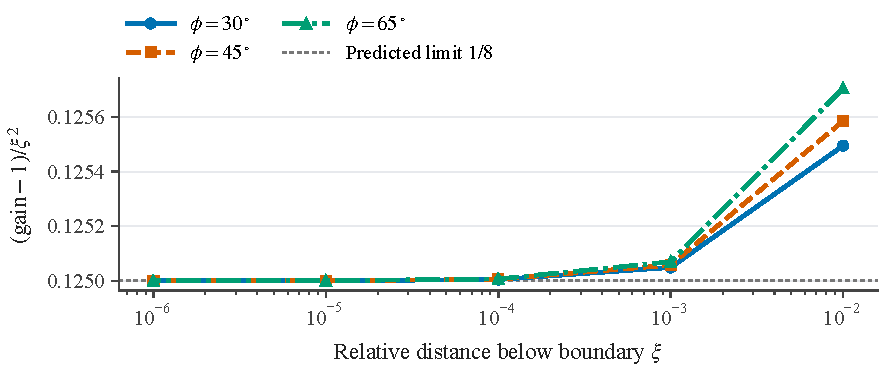
\includegraphics[width=.92\linewidth]{figures/boundary_coefficient.pdf}
\caption{The attainable two-phase gain approaches the sharp all-schedule coefficient $1/8$ near the boundary. Each curve fixes the angle and $B=4$, then varies the relative boundary distance. Values use 80-digit exponentials, not a fit to float64 cancellation.}\label{fig:near}
\end{figure}

The boundary curves in the main text use angles $30,45,65$ degrees; masses $0,10^{-4},10^{-3},10^{-2},0.1$; ridge $0.02$; and 100 budgets from $0.2$ to 12. Candidates include static mixing, the pure preparation rule when feasible, and a bounded scalar search over the mixed witness amplitude. These are attainable lower bounds on the optimal gain. No global optimizer is claimed below the exact boundary.

\subsection{Additive-noise checks}
For 480 cases with seed 921005, angles are uniform on $[0.2,1.4]$, budgets on $[0.1,20]$, masses in $\{0,0.001,0.1,1\}$, noise amplitudes in $\{0.01,0.1,0.3\}$, and phase counts in $\{1,2,5,20\}$. Ridge is 0.02. Each phase is solved through its symmetric eigendecomposition and the exact Ornstein--Uhlenbeck covariance integral. We record deterministic-plus-noise risk, the isolated noise contribution, and both theoretical lower bounds. No violations are observed. Separate curves fix $45^\circ$, zero orthogonal mass, ridge 0.02, and 121 budgets from 1 to 24 for $\sigma\in\{0,0.001,0.01,0.1\}$. The zero-noise gain ceiling is finite because it includes the energy lower bound, not only the vanishing determinant bound.

\begin{figure}[h]
\centering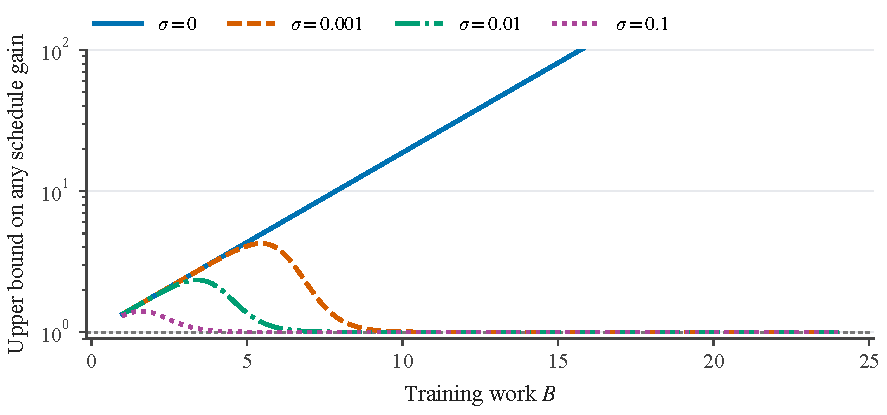
\includegraphics[width=.92\linewidth]{figures/diffusion_ceiling.pdf}
\caption{A global upper bound on the gain of any deterministic schedule in the stated additive-noise model. Positive isotropic noise eventually drives the ceiling to one. These are bounds, not achieved gains and not an SGD diffusion fit.}\label{fig:diffusion}
\end{figure}

\subsection{Exact expected Gaussian SGD}
The full grid has angles $30,45,65$ degrees, work $B\in\{1,4,8\}$, steps $\eta\in\{0.01,0.05\}$, batch sizes $m\in\{1,8,64\}$, label standard deviations $\sigma_y\in\{0,0.1\}$, and orthogonal masses $\varepsilon\in\{0,10^{-4},0.01,0.1\}$. Source covariance is \eqref{eq:mainfamily} with ridge 0.02. There are $K=B/\eta$ updates and $Km$ examples per comparison. We repeat the same 432 conditions for per-example and per-batch source selection. This yields 864 deterministic moment calculations; there is no finite-trial sampling error in their expected risks.

For each condition, the static comparator is the global lower/upper bracket of Appendix~\ref{app:moments}. Every recorded relative width is below $10^{-3}$. The schedule library consists of every integer pure-source switch in both orders, mixed witnesses with amplitude fractions $0.01,0.05,0.1,0.25,0.5,0.75,1$, and the best static grid point. Mixed witnesses split the updates as $\lfloor K/2\rfloor$ and $K-\lfloor K/2\rfloor$. Pure-switch risks are evaluated by composing exact moment operators, not by fitting an exponential. The flow-rule switch $\tau$ is rounded to the nearest update; it is reported separately when feasible (384 of 432 settings for each sampling convention).

Descriptive candidate and flow-rule gains use the best evaluated static risk (the upper bracket) in the numerator; gain counts use the lower bracket. The lower-bracket gain exceeding 1.01 occurs in 186 per-example and 220 per-batch settings. Their maximal candidate gains are 2.5855 and 8.9237, respectively; these maxima are descriptive and are not the headline evidence. Median gains and the full grid show the limited and noise-dependent nature of the improvements. The 18 aggregated conditions below include both successful and unsuccessful settings. The candidate library includes static mixing, so a median of one is a tie by construction, not evidence that every proposed curriculum is safe.
\begin{table}[h]\centering\small
\caption{Complete aggregated Gaussian SGD conditions. Each row includes 48 settings. Median gains use the upper static bracket; $>1\%$ counts use the lower bracket.}
\begin{tabular}{llrrrr}\toprule Sampling & Batch & $B$ & Median candidate & Median flow rule & $>1\%$ gains\\\midrule
batch & 1 & 1 & 1.0189 & 0.8783 & 42 \\
batch & 1 & 4 & 1.0000 & 0.7790 & 6 \\
batch & 1 & 8 & 1.0000 & 0.1932 & 0 \\
batch & 8 & 1 & 1.0209 & 0.8702 & 44 \\
batch & 8 & 4 & 1.3605 & 1.3574 & 28 \\
batch & 8 & 8 & 1.0000 & 0.3705 & 8 \\
batch & 64 & 1 & 1.0214 & 0.8698 & 44 \\
batch & 64 & 4 & 1.5414 & 1.5361 & 28 \\
batch & 64 & 8 & 1.0000 & 0.6407 & 20 \\
example & 1 & 1 & 1.0189 & 0.8783 & 42 \\
example & 1 & 4 & 1.0000 & 0.7790 & 6 \\
example & 1 & 8 & 1.0000 & 0.1932 & 0 \\
example & 8 & 1 & 1.0171 & 0.8688 & 40 \\
example & 8 & 4 & 1.0269 & 0.9891 & 25 \\
example & 8 & 8 & 1.0000 & 0.1787 & 0 \\
example & 64 & 1 & 1.0169 & 0.8682 & 40 \\
example & 64 & 4 & 1.1633 & 1.1627 & 28 \\
example & 64 & 8 & 1.0000 & 0.1844 & 5 \\
\bottomrule\end{tabular}\end{table}


\paragraph{Independent Monte Carlo validation.}
We fix $45^\circ$, ridge 0.02, $\varepsilon=0.001$, $\eta=0.05$, $B\in\{2,4\}$, $m\in\{1,8\}$, and $\sigma_y\in\{0,0.1\}$. Both sampling conventions are tested, with static and selected two-phase methods, yielding 32 conditions. Each uses 8,192 independent trajectories. Initial errors are $u\pm\sqrt\varepsilon v$ with equiprobable signs, so their second moment is exactly the theoretical input in expectation. Fresh Gaussian examples and independent noise are drawn at every update. Within each condition methods share a seed for paired comparisons, but trajectories are independent across the 8,192 replicates. Standard errors use the sample standard deviation of terminal losses divided by the square root of this replicate count. All 32 means lie within three standard errors of the exact risk; the largest absolute standardized discrepancy is 2.096. This is a model-implementation check, not a familywise statistical claim.

\paragraph{Oracle versus paid computation.}
The moment library assumes that the source covariances, label variance, and initial second moment are known. Search cost is not included in its work axis. It therefore measures whether a schedule helps the training dynamics under equal update/example counts. It does not establish a practical cost saving after estimating these moments. The separate paid-pilot experiment explicitly accounts for its own observation and declared planning costs, and retains its poor all-outcome performance.

\section{Supporting comparisons and paid decisions}
\begin{proposition}[Classical comparison consequences]\label{prop:obstructions}
If $G_A$ and $G_B$ commute, every fixed schedule equals its exposure-matched static mixture. For arbitrary symmetric PSD generators, if $S=Q=I$, every two-phase schedule has risk at least that of its exposure-matched static mixture. Consequently $\Rt=\Rs$ in the latter setting. More generally, if $S,Q$ are positive definite,
\begin{equation}
 1\le\Gamma_2(B)\le\kappa(S)\kappa(Q),\label{eq:kappa}
\end{equation}
where $\kappa$ is the spectral condition number.
\end{proposition}
For two phases, Golden--Thompson gives
\begin{equation}
 \norm{e^{-b_2G_2}e^{-b_1G_1}}_F^2
 =\tr(e^{-2b_1G_1}e^{-2b_2G_2})
 \ge\tr(e^{-2(b_1G_1+b_2G_2)}).
\end{equation}
This proves the isotropic case. Eigenvalue comparison proves \eqref{eq:kappa}; details appear in Appendix~\ref{app:basic}. The isotropic argument is a two-phase result, not an asserted multivariate Golden--Thompson inequality. Its practical message is simple: a nonzero commutator does not establish that a curriculum beats the best mixture.

\subsection{An exact global comparison}\label{sec:exact}
Choose $0<\phi<\pi/2$ and define
\begin{equation}
 c=\cos\phi,\quad a=(1+c)/2,\quad d=(1-c)/2,\quad
 u=\begin{pmatrix}\cos(\phi/2)\\\sin(\phi/2)\end{pmatrix},\quad
 v=\begin{pmatrix}-\sin(\phi/2)\\\cos(\phi/2)\end{pmatrix}.
\end{equation}
The source directions are $v_A=(1,0)^\top$ and $v_B=(\cos\phi,\sin\phi)^\top$. Set
\begin{equation}
 G_A=v_Av_A^\top+\rho I,\quad G_B=v_Bv_B^\top+\rho I,
 \quad S_\eps=uu^\top+\eps vv^\top,\quad Q=I,\label{eq:family}
\end{equation}
with $\rho\ge0$ and $\eps\ge0$. The initial error is concentrated along the bisector $u$; $\eps$ measures orthogonal second-moment mass. Positive $\rho$ makes both sources positive definite, so the advantage is not restricted to singular source Hessians.

\begin{theorem}[Budget-optimal static mixture]\label{thm:static}
For the family \eqref{eq:family}, every budget $B\ge0$ and every $\eps\ge0$,
\begin{equation}
 \boxed{\Rs(B,\eps)=\tfrac12e^{-2\rho B}
        \left(e^{-2aB}+\eps e^{-2dB}\right).}\label{eq:static}
\end{equation}
The constant mixture $p=1/2$ attains this value globally.
\end{theorem}
The proof uses more than symmetry: in the $(u,v)$ basis, every mixture has diagonal $(a+\rho,d+\rho)$. Scalar Jensen applied to each vector's spectral measure lower-bounds its exponential quadratic form by the corresponding diagonal exponential. The balanced mixture is diagonal and attains both bounds. This also yields a general common-diagonal lemma in Appendix~\ref{app:exact}.

Define
\begin{equation}
 \tau=\log\frac{1+c}{c},\qquad
 A_\phi=\frac{a}{c^2},\quad D_\phi=\frac{d(1+2c)^2}{c^2},\quad F_\phi=\frac{c^2}{a}=A_\phi^{-1}.
\end{equation}
The \emph{preparation curriculum} trains on $A$ for $\tau$ and on $B$ for $B-\tau$. Its first phase sends the bisector error exactly into the direction learned most rapidly by $B$.

\begin{theorem}[Constructive comparison and globally optimal rate]\label{thm:prep}
For $B\ge\tau$, the preparation risk is exactly
\begin{equation}
 \boxed{\Rp(B,\eps)=\tfrac12e^{-2\rho B}
 \left[(A_\phi+\eps D_\phi)e^{-2B}+\eps F_\phi\right].}\label{eq:prep}
\end{equation}
For $\eps=0$, it beats every static mixture whenever
$B>\log A_\phi/(2d)$, with loss ratio
\begin{equation}
 \frac{\Rs(B,0)}{\Rp(B,0)}=F_\phi e^{2dB}.\label{eq:ratio}
\end{equation}
Moreover, even arbitrary measurable schedules satisfy
\begin{equation}
 \tfrac12e^{-2(1+\rho)B}\le\Ra(B,0)
 \le\Rt(B,0)\le\tfrac{A_\phi}{2}e^{-2(1+\rho)B}.\label{eq:globalrate}
\end{equation}
Thus a two-phase construction achieves the globally optimal exponential rate, up to a constant independent of $B$.
\end{theorem}
Equation~\eqref{eq:globalrate} does not say the explicit switch time is the exact finite-budget optimum. The lower bound follows because no source has an eigenvalue exceeding $1+\rho$. The closed form follows by resolving the post-preparation residual into $v_B$ and its orthogonal complement.

\paragraph{Loss gains are not work gains.}
Let $B_s(\ell)$ and $B_p(\ell)$ be the work needed by the best static mixture and the preparation curriculum to reach loss $\ell$ at $\eps=0$. For sufficiently small $\ell$,
\begin{equation}
 B_s(\ell)=\frac{\log(1/(2\ell))}{2(\rho+a)},\quad
 B_p(\ell)=\frac{\log(A_\phi/(2\ell))}{2(\rho+1)},\quad
 \lim_{\ell\downarrow0}\frac{B_s(\ell)}{B_p(\ell)}
 =\frac{\rho+1}{\rho+a}<2.\label{eq:work}
\end{equation}
The same limiting work ratio holds for the optimal variable schedule by \eqref{eq:globalrate}. At $\phi=45^\circ$, $\rho=0$, the equal-work loss ratios are $1.8904$ at $B=4$ and $6.1003$ at $B=8$, but the limiting work ratio is only $1.1716$.

\subsection{Directional uncertainty changes the asymptotic answer}\label{sec:uncertainty}
An exact preparation can be useful without being robust. Equation~\eqref{eq:prep} shows what goes wrong: orthogonal initial-error mass leaves a residual term that the final rank-one source cannot remove. A common ridge shrinks this term, but does not remove the gap between its decay rate and that of the optimal mixture.

\begin{theorem}[Exact uncertainty boundary for preparation]\label{thm:threshold}
Restrict $0\le\eps\le1$. Assume $B\ge\tau$ and $N(B)=e^{-2aB}-A_\phi e^{-2B}>0$. Then preparation beats the globally best static mixture precisely when
\begin{equation}
 0\le\eps<\eps_{\mathrm{prep}}(B):=
 \frac{e^{-2aB}-A_\phi e^{-2B}}
 {F_\phi+D_\phi e^{-2B}-e^{-2dB}}.\label{eq:threshold}
\end{equation}
The denominator is positive and $\eps_{\mathrm{prep}}(B)\sim e^{-2aB}/F_\phi$ as $B\to\infty$. For $N(B)\le0$, preparation does not strictly improve over static mixing for any $\eps\in[0,1]$.
\end{theorem}
The final assertion follows by linear interpolation between the known-error and isotropic no-benefit cases (Appendix~\ref{app:uncertainty}). The threshold concerns this explicit schedule, not the entire two-phase class.



The next theorem goes beyond failure of the explicit schedule.
\begin{theorem}[Full-rank obstruction for every two-phase curriculum]\label{thm:fullrank}
For \eqref{eq:family} and $0<\eps\le1$,
\begin{equation}
 \frac{\eps c^2}{2}e^{-2(\rho+d)B}
 \le\Rt(B,\eps)\le\Rs(B,\eps)
 \le\frac{1+\eps}{2}e^{-2(\rho+d)B}.\label{eq:floor}
\end{equation}
Consequently
\begin{equation}
 \lim_{B\to\infty}-\frac{\log\Rt(B,\eps)}{2B}=\rho+d
 \quad(\eps>0),\qquad
 \lim_{B\to\infty}-\frac{\log\Rt(B,0)}{2B}=\rho+1.
\end{equation}
\end{theorem}
Every mixture has a slow eigenvalue at most $\rho+d$. Its slow eigenvector lies in a cone of angular width $\phi$, so the slow directions of any two phases have squared overlap at least $c^2$. A nonnegative two-eigenbasis expansion of the squared Frobenius norm then proves \eqref{eq:floor}. This is uniform over both phase lengths and both mixture weights. It does not require optimizing them numerically.

The two-phase bound above is retained as a separate elementary comparison. Theorem~\ref{thm:general_boundary} strengthens it to eventual exact static optimality for every measurable schedule in this family.

\begin{corollary}[Sharp peak-gain law for the explicit curriculum]\label{cor:peak}
Fix $\phi$. As $\eps\downarrow0$,
\begin{equation}
 \sup_{B\ge\tau}\frac{\Rs(B,\eps)}{\Rp(B,\eps)}
 \sim a^a d^d A_\phi^{-c}\,\eps^{-d}.\label{eq:peak}
\end{equation}
\end{corollary}
Thus uncertainty limits not only how long the explicit schedule is useful, but also its largest attainable loss advantage. This peak law is not a matching characterization of the optimal two-phase gain at every positive $\eps$.

\subsection{When shared curricula cannot change a power-law exponent}\label{sec:spectral}
The finite-dimensional exponential comparison does not automatically imply an improved neural scaling exponent. Consider independent blocks $j\ge1$, with initial masses $w_j=\tr S_j\asymp j^{-1-\beta}$ and scales $\lambda_j\asymp j^{-\alpha}$, where $\alpha,\beta>0$. All blocks receive \emph{one common} allocation $p(t)$. Assume constants $L,m>0$ and one fixed $p_0$ such that
\begin{equation}
 0\preceq G_{i,j}\preceq L\lambda_j I\quad(i=A,B),\qquad
 G(p_0)_j\succeq m\lambda_j I\quad\text{for every }j.\label{eq:envelope}
\end{equation}
The evaluation geometry is identity. With capacity $J$, only the first $J$ blocks train; the remaining mass is included as an unlearned tail. These assumptions describe comparable learning rates across spectral scales, not a guarantee for arbitrary source geometries.

\begin{theorem}[Shared-schedule and capacity-work exponents]\label{thm:spectral}
Under \eqref{eq:envelope}, for $B\ge1$, $J\ge1$, the optimal risk over all shared measurable schedules and the risk of the static mixture $p_0$ satisfy the same bounds up to constants:
\begin{equation}
 \R^*(B,J)\asymp B^{-\beta/\alpha}+J^{-\beta}.
\end{equation}
In the infinite-capacity limit the rate is $B^{-\beta/\alpha}$. If capacity is chosen before training and total normalized model work is $C=JB$, then
\begin{equation}
 \inf_{JB\le C}\R^*(B,J)\asymp C^{-\beta/(\alpha+1)},\label{eq:capacity}
\end{equation}
attained by $J\asymp C^{1/(\alpha+1)}$ and $B\asymp C^{\alpha/(\alpha+1)}$. The static mixture attains the same exponent.
\end{theorem}
The lower bound applies to all schedules because block $j$ cannot contract faster than $L\lambda_j$. The static mixture contracts every block at rate at least $m\lambda_j$. A tail-sum comparison and balancing capacity against training work finish the proof. This is not a statement that curricula give no constant-factor gains. It also does not allow a different switch time in every block, change the optimizer, or grow capacity during training.



\subsection{From an oracle schedule to a paid acceptance certificate}\label{sec:certificate}
The preceding theorems assume known geometry. To distinguish a favorable oracle comparison from an actionable decision, first consider approximate generators and second moments. Suppose both true and estimated generators are PSD, $\norm{G_i-\widehat G_i}_{\op}\le\delta_G$ and $\norm{S-\widehat S}_*\le\delta_S$, where $\norm{\cdot}_*$ is nuclear norm. For $Q=I$, every fixed schedule of duration $T$ obeys
\begin{equation}
 |\R(\pi)-\widehat\R(\pi)|\le
 r_T:=\tfrac12\delta_S+\tr(\widehat S)\min\{2,T\delta_G\}.\label{eq:uniform}
\end{equation}
Duhamel's identity proves this uniformly over schedules (Appendix~\ref{app:certificate}). An $\eta$-approximate empirical minimizer over a candidate library has excess risk at most $2r_T+\eta$ relative to that library at duration $T$. This is not a guarantee relative to a competitor trained for a larger, uncharged budget.

\paragraph{Charge the observation before comparing.}
Our implemented pilot addresses a more specific problem: the source generators are known but a deterministic residual $e$ is unknown. It observes $n$ independent $N(e_j,\sigma^2)$ measurements of each coordinate. In dimension $D$, with probability at least $1-\delta$,
\begin{equation}
 \norm{e-\widehat e}\le r=\frac{\sigma}{\sqrt n}
       \left(\sqrt D+\sqrt{2\log(1/\delta)}\right).\label{eq:gaussian}
\end{equation}
This is a direct coordinate-measurement model, not an assertion that a neural-network residual is freely observable. The pilot costs $Dnq$ at query price $q$, and the planner is assigned cost $h$. Only $T=B-Dnq-h$ remains for training.

For a known candidate transition $\Phi$, convex quadratic expansion gives a valid upper bound
\begin{equation}
 U_\Phi=\tfrac12\norm{\Phi\widehat e}^2
 +r\norm{\Phi^\top\Phi\widehat e}
 +\tfrac12r^2\norm{\Phi}_{\op}^2.\label{eq:upper}
\end{equation}
Appendix~\ref{app:envelope} constructs a uniform lower bound $L_s(B)$ on the risk of \emph{every static mixture trained for the full original budget}, using a grid of cells and a within-cell matrix-exponential bound. The certificate accepts a candidate trained for $T$ only when
\begin{equation}
 U_\Phi(T)<L_s(B).\label{eq:gate}
\end{equation}

\begin{proposition}[Paid acceptance guarantee]\label{prop:accept}
On the confidence event \eqref{eq:gaussian}, every candidate accepted by \eqref{eq:gate}, including one selected after observing the pilot, has lower population risk than the optimal no-pilot static mixture trained for $B$. Rejection carries no such guarantee: the pilot cost has already been spent.
\end{proposition}
The proof is the chain $\R(\Phi)\le U_\Phi<L_s\le\Rs(B)$. The substantive requirements are simultaneous bounds over the selection set and correct budget accounting. The implementation uses float64 with explicit numerical padding, not directed-rounding interval arithmetic. Its mathematical certificate is valid in real arithmetic; its numerical output is not a formal computer-verified proof.


\section{Basic comparison proofs}\label{app:basic}
\paragraph{Notation.} All matrix norms without a subscript are Euclidean operator norms, except $\norm{\cdot}_F$ and $\norm{\cdot}_*$. Risk is one half of the stated quadratic form. The budget variable is $B$, while $d=(1-\cos\phi)/2$ is the slow eigenvalue of the balanced, unregularized mixture. A second moment need not be a centered covariance.

\begin{proof}[Proof of Proposition~\ref{prop:obstructions}]
If $G_A$ and $G_B$ commute, all their convex combinations commute. A product of exponentials is the exponential of their sum. The same identity holds for measurable schedules by simultaneous diagonalization and solving each scalar equation. Its effective mixture weight is $B^{-1}\int_0^B p(t)\,dt$ for $B>0$; the zero-budget statement is immediate.

For two phases let $X=b_1G_1$, $Y=b_2G_2$, $\Phi=e^{-Y}e^{-X}$, and $\Psi=e^{-(X+Y)}$. Cyclicity of trace gives
\[
 \norm{\Phi}_F^2=\tr(e^{-2X}e^{-2Y}).
\]
Golden--Thompson, applied to the symmetric matrices $-2X$ and $-2Y$, gives $\norm\Phi_F^2\ge\tr(e^{-2(X+Y)})=\norm\Psi_F^2$. The exponent $X+Y$ equals $BG(\bar p)$, with $\bar p=(b_1p_1+b_2p_2)/B$. Thus $\Psi$ is a feasible static comparator. Since static schedules belong to the two-phase class, their optimized risks coincide in the isotropic setting.

For positive definite $S,Q$, denote their smallest and largest eigenvalues by $s_-,s_+,q_-,q_+$. For every matrix $M$,
\[
 \tfrac12q_-s_-\norm M_F^2\le\tfrac12\tr(QMSM^\top)
 \le\tfrac12q_+s_+\norm M_F^2.
\]
Applying the upper bound to the exposure-matched static transition and the lower bound to the curriculum gives
$\R(\Psi)\le\kappa(Q)\kappa(S)\R(\Phi)$.
The optimal static risk is at most $\R(\Psi)$ for each curriculum. Taking the infimum over two-phase curricula proves the ratio bound. No product inequality with three or more independent exponents is used.
\end{proof}

\section{Exact static optimum and preparation formula}\label{app:exact}
\begin{lemma}[Common-diagonal static benchmark]\label{lem:diagonal}
Suppose symmetric generators $G_i$ have the same diagonal $(\gamma_1,\ldots,\gamma_D)$ in an orthonormal basis $(u_j)$. Suppose their convex hull contains $G_0=\sum_j\gamma_ju_ju_j^\top$, and $S=\sum_j s_ju_ju_j^\top$ with $s_j\ge0$. For $Q=I$, $G_0$ globally minimizes static risk at every $B\ge0$, with value $\frac12\sum_js_je^{-2B\gamma_j}$.
\end{lemma}
\begin{proof}
For a static generator $G$ with eigenpairs $(\lambda_k,z_k)$,
\[
 u_j^\top e^{-2BG}u_j=\sum_k (u_j^\top z_k)^2e^{-2B\lambda_k}
 \ge \exp\left(-2B\sum_k(u_j^\top z_k)^2\lambda_k\right)
 =e^{-2B\gamma_j}.
\]
The weights are nonnegative and sum to one. The inequality is scalar Jensen for the convex function $x\mapsto e^{-2Bx}$. Summing against $s_j/2$ gives the lower bound. The diagonal generator $G_0$ attains it. This is a direct spectral Jensen consequence; operator convexity of the exponential is neither assumed nor needed.
\end{proof}

\begin{proof}[Proof of Theorem~\ref{thm:static}]
In the $(u,v)$ basis, $G(p)-\rho I$ has the form
\begin{equation}
 \begin{pmatrix}a&z(p)\\z(p)&d\end{pmatrix},\qquad
 z(p)=(1-2p)\sqrt{ad}.\label{eq:bisector_matrix}
\end{equation}
Indeed $u^\top v_A=u^\top v_B=\sqrt a$, whereas $v^\top v_A=-\sqrt d$ and $v^\top v_B=\sqrt d$. The diagonal is independent of $p$, and the off-diagonal vanishes at $p=1/2$. Apply Lemma~\ref{lem:diagonal} with masses $1,\eps$.
\end{proof}

\begin{proof}[Proof of the formula in Theorem~\ref{thm:prep}]
The common ridge commutes with all terms, so every transition is multiplied by $e^{-\rho B}$. It suffices to compute at $\rho=0$. In the original source basis, $u=(\sqrt a,\sqrt d)^\top$ and $v=(-\sqrt d,\sqrt a)^\top$. Since $e^{-\tau}=c/(1+c)=c/(2a)$,
\[
 e^{-\tau v_Av_A^\top}u
 =\begin{pmatrix}c/(2\sqrt a)\\\sqrt d\end{pmatrix}
 =\frac{v_B}{2\sqrt a}.
\]
The identity uses $\sin\phi=2\sqrt{ad}$. Thus the squared norm after the second phase is
\[
 \norm{e^{-(B-\tau)v_Bv_B^\top}e^{-\tau v_Av_A^\top}u}^2
 =\frac{e^{-2(B-\tau)}}{4a}=\frac{a}{c^2}e^{-2B}=A_\phi e^{-2B}.
\]
For the orthogonal vector, define $w=e^{-\tau v_Av_A^\top}v=(-c\sqrt d/(2a),\sqrt a)^\top$ and $v_B^\perp=(-\sin\phi,\cos\phi)^\top$. Direct inner products give
\[
 (v_B^\top w)^2=\frac{d(1+2c)^2}{(1+c)^2},\qquad
 ((v_B^\perp)^\top w)^2=\frac{c^2}{a}=F_\phi.
\]
The parallel component is multiplied by $e^{-2(B-\tau)}$ and the perpendicular component is unchanged. Therefore its final squared norm is $D_\phi e^{-2B}+F_\phi$. Weighting the two initial components by $1$ and $\eps$, dividing by two, and restoring $e^{-2\rho B}$ proves \eqref{eq:prep}.
\end{proof}

\begin{proof}[Proof of the rate and work claims]
At $\eps=0$, dividing \eqref{eq:static} by \eqref{eq:prep} gives $F_\phi e^{2(1-a)B}=F_\phi e^{2dB}$. Strict improvement is equivalent to $2dB>\log A_\phi$ whenever the preparation schedule is feasible.

For every admissible allocation, $G(p(t))\preceq(1+\rho)I$. The scalar energy derivative satisfies
\[
 \frac{d}{dt}\norm{e(t)}^2=-2e(t)^\top G(p(t))e(t)
 \ge-2(1+\rho)\norm{e(t)}^2.
\]
Integration gives $\norm{e(B)}^2\ge e^{-2(1+\rho)B}\norm{e(0)}^2$. The initial vector $u$ has unit norm. This proves the lower bound for arbitrary measurable schedules; the explicit schedule supplies the upper bound. The bounds imply the same exponential rate for $\Rt$ and $\Ra$.

Solving the two explicit risk formulas for their first crossing of a sufficiently small $\ell$ gives \eqref{eq:work}. The preparation crossing eventually exceeds $\tau$. For the optimal arbitrary schedule, the lower and upper rate bounds bracket the required work between $\log(1/(2\ell))/(2(1+\rho))$ and $\log(A_\phi/(2\ell))/(2(1+\rho))$. Their difference is constant in $\ell$, so they give the same limiting static-to-curriculum work ratio.
\end{proof}

\section{Uncertainty thresholds, rate obstruction, and peak law}\label{app:uncertainty}
\begin{proof}[Proof of Theorem~\ref{thm:threshold}]
Subtracting the two exact formulas yields
\[
 2e^{2\rho B}(\Rs-\Rp)=N(B)-\eps K(B),\qquad
 K(B)=F_\phi+D_\phi e^{-2B}-e^{-2dB}.
\]
At $\eps=1$, Proposition~\ref{prop:obstructions} implies $N(B)-K(B)\le0$, since the preparation curriculum is a two-phase schedule and the balanced static mixture is optimal. If $N(B)>0$, it follows that $K(B)\ge N(B)>0$, and strict improvement is exactly $\eps<N(B)/K(B)$. This threshold is at most one. As $B\to\infty$, $N(B)\sim e^{-2aB}$ and $K(B)\to F_\phi>0$, proving the asymptotic expression. If $N(B)\le0$, the difference is nonpositive both at $\eps=0$ and at $\eps=1$. Affinity in $\eps$ proves nonpositivity throughout $[0,1]$. No assertion for $\eps>1$ is required for this threshold statement.
\end{proof}

\begin{lemma}[Slow-eigenvector cone]\label{lem:cone}
For all $p\in[0,1]$, the smaller eigenvalue of $G(p)$ in \eqref{eq:family} is at most $\rho+d$. Its unit slow eigenvector can be chosen to make angle at most $\phi/2$ with $v$, and slow eigenvectors for any two mixtures have squared inner product at least $c^2$.
\end{lemma}
\begin{proof}
In \eqref{eq:bisector_matrix}, $a-d=c>0$ and $|z(p)|\le\sqrt{ad}=\sin\phi/2$. The smaller eigenvalue is
\[
 \mu_-(p)=\rho+\frac{1-\sqrt{c^2+4z(p)^2}}{2}\le\rho+\frac{1-c}{2}=\rho+d.
\]
Diagonalization rotates the principal axes by an angle $\psi$ satisfying $|\tan(2\psi)|=2|z|/c\le\tan\phi$, with $|2\psi|<\pi/2$. Hence $|\psi|\le\phi/2$. The slow axes lie in an angular cone of width $\phi<\pi/2$, and consistently oriented unit vectors have inner product at least $\cos\phi=c$.
\end{proof}

\begin{proof}[Proof of Theorem~\ref{thm:fullrank}]
Let phase generators $G_1,G_2$ have orthonormal eigenvectors $w_{1,k},w_{2,l}$ and eigenvalues $\mu_{1,k},\mu_{2,l}$. For $\Phi=e^{-b_2G_2}e^{-b_1G_1}$, expand the trace as
\begin{equation}
 \norm\Phi_F^2=\sum_{k,l}
 e^{-2b_1\mu_{1,k}-2b_2\mu_{2,l}}
 |w_{1,k}^\top w_{2,l}|^2.\label{eq:nonnegative_expansion}
\end{equation}
Every term is nonnegative. Keep only the slow--slow term and apply Lemma~\ref{lem:cone} to obtain
$\norm\Phi_F^2\ge c^2e^{-2(\rho+d)(b_1+b_2)}$.
For $0<\eps\le1$, $S_\eps\succeq\eps I$, so $\R(\Phi)\ge\eps\norm\Phi_F^2/2$. This proves the uniform lower bound over all two-phase durations and mixture weights. The upper bound follows from the exact static formula and $a>d$. Taking logarithms and dividing by $-2B$ proves the rate for fixed positive $\eps$. The $\eps=0$ statement follows from Theorem~\ref{thm:prep}. The constants in the positive-$\eps$ lower bound vanish as $\eps\downarrow0$, which is why these limits do not commute.
\end{proof}

\begin{proposition}[Arbitrary-stage volume obstruction]\label{prop:volume}
For \eqref{eq:family}, $\eps>0$, and every measurable schedule,
\begin{equation}
 \R(\pi)\ge\sqrt\eps\,e^{-(1+2\rho)B}.
\end{equation}
\end{proposition}
\begin{proof}
The trace of every generator is $1+2\rho$. Liouville's determinant formula gives $\det\Phi_\pi=e^{-(1+2\rho)B}$. The two eigenvalues of $\Phi_\pi S_\eps\Phi_\pi^\top$ are positive, with product $\eps e^{-2(1+2\rho)B}$. Arithmetic--geometric mean bounds their sum below by twice the square root of this product. Dividing by two proves the result. This does not imply the sharper two-phase exponent $\rho+d$ for arbitrary schedules.
\end{proof}

\begin{proof}[Proof of Corollary~\ref{cor:peak}]
Put $x=e^{-2B}$, $A_\eps=A_\phi+\eps D_\phi$, and suppress the fixed angle subscript on $F$. The ratio is
\[
 \frac{x^a+\eps x^d}{A_\eps x+\eps F},\qquad
 0<x\le e^{-2\tau},\quad a+d=1.
\]
For $f(x)=x^a/(A_\eps x+\eps F)$, differentiation shows its unique unrestricted maximum is at
\[
 x_*=\frac{a\eps F}{d A_\eps},\qquad
 f(x_*)=a^ad^dA_\eps^{-a}F^{-d}\eps^{-d}.
\]
For sufficiently small $\eps$, $x_*$ lies in the admissible interval. The second summand $g(x)=\eps x^d/(A_\eps x+\eps F)$ is uniformly $O(\eps^d)$: substitute $x=\eps t$ and use boundedness of $t^d/(A_\eps t+F)$ on $t>0$, uniformly as $\eps\downarrow0$. Consequently the maximum of $f+g$ differs from the maximum of $f$ by at most $O(\eps^d)$. Since $F=A_\phi^{-1}$ and $a-d=c$, the leading constant converges to $a^ad^dA_\phi^{-a+d}=a^ad^dA_\phi^{-c}$.
\end{proof}

\begin{figure}[t]
\centering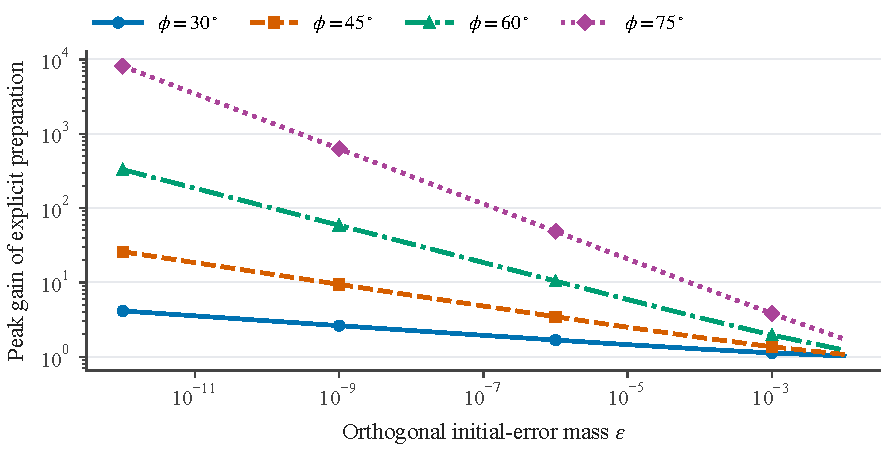
\includegraphics[width=.92\linewidth]{figures/peak_gain.pdf}
\caption{The peak preparation gain grows as orthogonal uncertainty decreases. The exponent is $d=(1-\cos\phi)/2$, so the gain can increase slowly when the source directions are close. The plotted maxima are one-dimensional numerical evaluations of the exact formulas; Corollary~\ref{cor:peak} is analytic.}\label{fig:peak}
\end{figure}

\section{Spectral and capacity-work proof}\label{app:spectral}
\begin{lemma}[Power-law exponential tail sum]\label{lem:tail}
For fixed $\alpha,\beta,k>0$,
\[
 \sum_{j\ge1}j^{-1-\beta}e^{-kBj^{-\alpha}}\asymp B^{-\beta/\alpha}
 \quad(B\ge1).
\]
The same conclusion holds when the weights and scales are comparable, with fixed positive constants, to $j^{-1-\beta}$ and $j^{-\alpha}$.
\end{lemma}
\begin{proof}
Write $J_B=\lceil B^{1/\alpha}\rceil$. For $j\ge J_B$, the exponential is bounded below by a positive constant depending only on $k,\alpha$, and the tail sum is comparable to $J_B^{-\beta}$. This proves the lower bound. For the upper bound, the same tail is at most a constant times $J_B^{-\beta}$. Partition $1\le j<J_B$ into dyadic bands with $j$ between $2^{-l-1}J_B$ and $2^{-l}J_B$, omitting empty bands. The total weight of a band is at most a constant times $J_B^{-\beta}2^{(l+1)\beta}$, while its exponential is at most $\exp(-k'2^{l\alpha})$ for a fixed $k'>0$. The series over bands converges independently of $B$, because exponential decay in $2^{l\alpha}$ dominates the geometric factor. Comparability changes only constants.
\end{proof}

\begin{proof}[Proof of Theorem~\ref{thm:spectral}]
For every trained block and every schedule, the energy differential inequality gives
\[
 \norm{e_j(B)}^2\ge e^{-2L\lambda_jB}\norm{e_j(0)}^2.
\]
Expectation gives the same bound with initial mass $w_j$. The proposed static mixture gives the upper bound $\E\norm{e_j(B)}^2\le e^{-2m\lambda_jB}w_j$. Hence
\[
 \tfrac12\sum_{j\le J}w_je^{-2L\lambda_jB}+\tfrac12\sum_{j>J}w_j
 \le\R^*(B,J)
 \le\tfrac12\sum_{j\le J}w_je^{-2m\lambda_jB}+\tfrac12\sum_{j>J}w_j.
\]
The lower expression is at least the full exponential sum, because each untrained tail term is at least its exponentially damped version. It is also at least the untrained mass. Lemma~\ref{lem:tail} and $\sum_{j>J}w_j\asymp J^{-\beta}$ therefore give a constant times $B^{-\beta/\alpha}+J^{-\beta}$ as a lower bound, using $\max(x,y)\ge(x+y)/2$. The upper expression is at most the full exponential sum plus the tail, proving the corresponding upper bound. In particular, no interchange of an unbounded number of blocks with a block-specific schedule is involved.

For total work $JB\le C$, the lower bound gives, up to constants,
\[
 B^{-\beta/\alpha}+J^{-\beta}
 \ge B^{-\beta/\alpha}+(B/C)^\beta.
\]
The two terms balance at $B\asymp C^{\alpha/(\alpha+1)}$. Either side of that scale is bounded below by a constant times $C^{-\beta/(\alpha+1)}$. Taking $J$ to be an integer within a constant factor of $C^{1/(\alpha+1)}$ and using the common static mixture gives the matching upper bound. The cost counts a fixed capacity during training; it is not a result about dynamically activating features.
\end{proof}

\section{Perturbation, discretization, and statistical bounds}\label{app:certificate}
\begin{lemma}[Uniform transition perturbation]\label{lem:duhamel}
Suppose two time-dependent symmetric PSD generators differ in operator norm by at most $\delta_G$ almost everywhere on $[0,T]$. Their transitions satisfy
$\norm{\Phi(T)-\widehat\Phi(T)}\le\min\{2,T\delta_G\}$.
\end{lemma}
\begin{proof}
All subinterval transitions are contractions. Variation of constants gives
\[
 \Phi(T)-\widehat\Phi(T)=
 -\int_0^T\Phi(T,s)(G(s)-\widehat G(s))\widehat\Phi(s,0)\,ds.
\]
The integral norm is at most $T\delta_G$. The triangle inequality and contraction bounds also give two. For source estimates with per-source errors bounded by $\delta_G$, every common convex allocation has an error at most $\delta_G$. Thus this result is simultaneous over schedules.
\end{proof}

\begin{proof}[Uniform risk and oracle bounds]
For $Q=I$, split the risk difference by first replacing $S$ by $\widehat S$ and then replacing $\Phi$ by $\widehat\Phi$. The covariance term has absolute value at most $\delta_S/2$, since $\norm{\Phi^\top\Phi}\le1$. If $\eta_\Phi=\norm{\Phi-\widehat\Phi}$, then
\[
 \norm{\Phi^\top\Phi-\widehat\Phi^\top\widehat\Phi}
 \le(\norm\Phi+\norm{\widehat\Phi})\eta_\Phi\le2\eta_\Phi.
\]
Because $\widehat S\succeq0$, the remaining risk difference is at most $\tr(\widehat S)\eta_\Phi$. Apply Lemma~\ref{lem:duhamel} to obtain \eqref{eq:uniform}.

If an empirical library minimizer has tolerance $\eta$, compare its true risk to its estimated risk, use empirical optimality, and compare the selected reference's estimated risk to its true risk. The two estimation differences contribute at most $2r_T$, proving the oracle inequality. An infimum can replace an attained optimum by an arbitrarily small additional tolerance. All terms use the same post-pilot budget $T$.
\end{proof}

\paragraph{Robustness of a strict comparison.}
For a nominal schedule with gap $\Delta=\R_{\mathrm{stat},0}^*(B)-\R_0(\pi)>0$, a uniform radius $r_B$ for both schedule and static risks gives
$\Rs(B)-\R(\pi)\ge\Delta-2r_B$.
Thus every positive nominal gap has a nonempty neighborhood of source/second-moment perturbations in which the comparison persists. This is an absolute-risk statement. Since the gap can be exponentially small, it is not a uniform large-budget robustness guarantee. The experiment records this conservative certificate separately from actual perturbed gains.

\begin{lemma}[Euler-to-flow bound at a specified schedule]\label{lem:euler}
Suppose every step uses a symmetric PSD generator with norm at most $L$, the common step size is $\eta$ with $\eta L\le1$, and there are $K$ steps, with total work $B=K\eta$. The Euler transition product and the exact piecewise-constant flow with the same stepwise allocation differ by at most $B\eta L^2/2$ in operator norm.
\end{lemma}
\begin{proof}
For $x\in[0,1]$, $0\le e^{-x}-(1-x)\le x^2/2$. Spectral calculus therefore bounds each one-step discrepancy by $\eta^2L^2/2$. Both the Euler factor and the exponential factor have norm at most one. A telescoping product identity bounds the total discrepancy by the sum of one-step discrepancies, namely $K\eta^2L^2/2$. Rounding a phase boundary is a separate change in the schedule; the experiment compares flow and Euler using identical rounded durations.
\end{proof}

\paragraph{Gaussian observation event.}
In the direct coordinate-query model, $\widehat e-e$ has law $(\sigma/\sqrt n)Z$ with $Z\sim N(0,I_D)$. Gaussian concentration for the 1-Lipschitz Euclidean norm gives $\Pr(\norm Z\ge\E\norm Z+t)\le e^{-t^2/2}$; Jensen gives $\E\norm Z\le\sqrt D$. Choosing $t=\sqrt{2\log(1/\delta)}$ yields \eqref{eq:gaussian}. These are classical concentration tools \citep{boucheron2013}. Candidate selection does not require a union bound when all candidate risks are bounded on this same state-ball event.

\section{Uniform static envelopes and the paid gate}\label{app:envelope}
This section supplies the global lower comparator used by the pilot. It is not needed for the exact-family optimum. Consider known generators, fixed full budget $B$, and $E(p)=e^{-BG(p)}$. Partition $[0,1]$ into cells centered at $q$ with half-width $h_q$. Let $m_q$ be the minimum of the smallest eigenvalues of the two endpoint generators. Concavity of the smallest eigenvalue implies $G(p)\succeq m_q I$ throughout the cell. Duhamel's formula then gives
\begin{equation}
 \norm{E(p)-E(q)}\le\eta_q:=B\norm{G_A-G_B}h_qe^{-Bm_q}.\label{eq:cell}
\end{equation}
Both generators along the interpolation have the stated lower bound, so the two exponential factors in the integral contribute $e^{-Bm_q}$. If true and estimated source generators differ by at most $\delta_G$, one can add $\min\{2,B\delta_G\}$ to $\eta_q$ by a triangle inequality.

Write $N=\norm{\widehat e}$, $y_q=E(q)\widehat e$, $n_q=\norm{E(q)}$, and $n_q^+=\min\{1,n_q+\eta_q\}$. On the state ball $\norm{e-\widehat e}\le r$, the triangle inequality supplies the cell-wise lower bound
\begin{equation}
 L_q^{\mathrm{amp}}=\tfrac12
 \left[\norm{y_q}-n_qr-\eta_q(N+r)\right]_+^2.\label{eq:amplower}
\end{equation}
A usually sharper bound follows from convexity of $f_p(e)=\norm{E(p)e}^2/2$:
\[
 f_p(e)\ge f_p(\widehat e)-r\norm{E(p)^2\widehat e}.
\]
The first term is bounded below by $\frac12[\norm{y_q}-\eta_qN]_+^2$. To bound the gradient norm, use
\[
 (E(p)^2-E(q)^2)\widehat e
 =E(p)(E(p)-E(q))\widehat e+(E(p)-E(q))y_q.
\]
Hence a second cell-wise lower bound is
\begin{equation}
 L_q^{\mathrm{dir}}=\tfrac12[\norm{y_q}-\eta_qN]_+^2
 -r\left(\norm{E(q)y_q}+\eta_q(\norm{y_q}+n_q^+N)\right).
\end{equation}
It follows that
\begin{equation}
 L_s(B)=\max\left\{0,\min_q\max\{L_q^{\mathrm{amp}},L_q^{\mathrm{dir}}\}\right\}
 \le\inf_{p\in[0,1]}\tfrac12\norm{E(p)e}^2.\label{eq:uniformlower}
\end{equation}
The bounds cover the whole cell rather than only its center, so optimizing on a grid does not invalidate the comparator.

\paragraph{Candidate upper bound.}
For $e=\widehat e+z$ with $\norm z\le r$, expand
\[
 \tfrac12\norm{\Phi e}^2
 =\tfrac12\norm{\Phi\widehat e}^2+
 z^\top\Phi^\top\Phi\widehat e+\tfrac12z^\top\Phi^\top\Phi z.
\]
Cauchy--Schwarz proves \eqref{eq:upper}. The amplitude bound $\frac12(\norm{\Phi\widehat e}+r\norm\Phi)^2$ is also valid, and the implementation takes the smaller bound. If an estimated transition has error $\eta_\Phi$, its directional bound can be enlarged by
$\frac12\eta_\Phi(2\norm{\widehat\Phi}+\eta_\Phi)(N+r)^2$.

\paragraph{Decision and budget.}
Each candidate may have a different remaining training budget if its additional cost differs. A valid upper bound uses that actual remaining budget. The baseline lower bound always uses the full original $B$. Taking the smallest candidate upper bound is valid on the common confidence event. If it is below \eqref{eq:uniformlower}, the accepted candidate beats every full-budget static mixture. This proves Proposition~\ref{prop:accept}. A static fallback after rejection has only $T$ training work, not $B$, so a claim of unconditional no-regression would be false.

\paragraph{Numerical status.}
The real-arithmetic statements above are inequalities. The supplied implementation computes eigendecompositions in float64 and pads bounds outward by $10^{-12}$. Padding is a precaution, not a proof of every floating-point operation's rounding error. The exact comparison theorems rely on analytic formulas, independently checked with 70-digit matrix exponentials; the pilot code remains a numerical realization of a mathematical certificate. A formally machine-verified gate would require directed-rounding linear algebra or a separately proved floating-point error bound.

\section{Experimental protocols and complete condition-level results}\label{app:experiments}
All data are generated within the release. The raw CSVs include failed or unfavorable comparisons as well as favorable ones. The theoretical family uses a unit-norm bisector error; its numbers should not be confused with unnormalized illustrative examples. Population linear risk is $\norm{\theta-\theta^*}^2/2$ under identity target covariance.

\subsection{Exact and robustness suites}
The exact family sweep uses source angles $15,30,45,60,75$ degrees; orthogonal masses $0,10^{-6},10^{-4},10^{-2},1$; ridges $0,0.05$; and 61 budgets between $\max\{1,\tau\}$ and 16. The static audit uses five angles, four masses, two ridges, and five budgets, comparing the analytic optimum to 101 weights spanning $[0,1]$. Its numerical grid is an audit, not the source of the optimality claim.

The isotropic suite draws 160 independent pairs of Wishart-like PSD matrices, with dimensions cycling through 2, 4, 8, and 12. Durations are uniform on $[0.02,3]$, and phase weights are uniform on $[0,1]$. The full-rank bound suite draws 400 two-phase schedules with angles in $[0.1,1.5]$ radians, log-uniform masses in $[10^{-6},1]$, ridges in $[0,0.2]$, and budgets in $[0.1,25]$. The code records absolute inequality margins, not an arbitrarily rounded success flag.

Perturbation tests independently rotate both source vectors and the initial vector by Gaussian angles with standard deviation $0$, $0.001$, $0.01$, $0.05$, or $0.1$ radians. Each condition has 24 seeds at budgets 4 and 8. The schedule retains the nominal $45^\circ$ preparation time. The static comparator uses a 257-point grid followed by a bounded scalar refinement near its best grid point, and is labeled a numerical comparator rather than a certified global optimum for perturbed inputs. The aggregate results are in Table~\ref{tab:perturb}.

\begin{table}[h]
\centering\small
\caption{Perturbed geometry: preparation gain against the numerical static comparator.}\label{tab:perturb}
\begin{tabular}{rrrrr}\toprule
Budget & Angular standard deviation & Median gain & Wins & Cases\\\midrule
4 & 0 & 1.8904 & 24 & 24 \\
4 & 0.001 & 1.8880 & 24 & 24 \\
4 & 0.01 & 1.7313 & 24 & 24 \\
4 & 0.05 & 0.6871 & 10 & 24 \\
4 & 0.1 & 0.2109 & 4 & 24 \\
8 & 0 & 6.1003 & 24 & 24 \\
8 & 0.001 & 2.0728 & 16 & 24 \\
8 & 0.01 & 0.0336 & 5 & 24 \\
8 & 0.05 & 0.0014 & 1 & 24 \\
8 & 0.1 & 0.0003 & 0 & 24 \\
\bottomrule\end{tabular}
\end{table}

The Euler check uses step sizes $0.2,0.1,0.05,0.025,0.0125$, budgets 2, 4, 8, and ridge 0.05. The switch is rounded to the nearest step for \emph{both} exact flow and Euler dynamics. Thus the measured operator discrepancy tests Lemma~\ref{lem:euler}, not an unaccounted switch-time error.

\begin{figure}[t]
\centering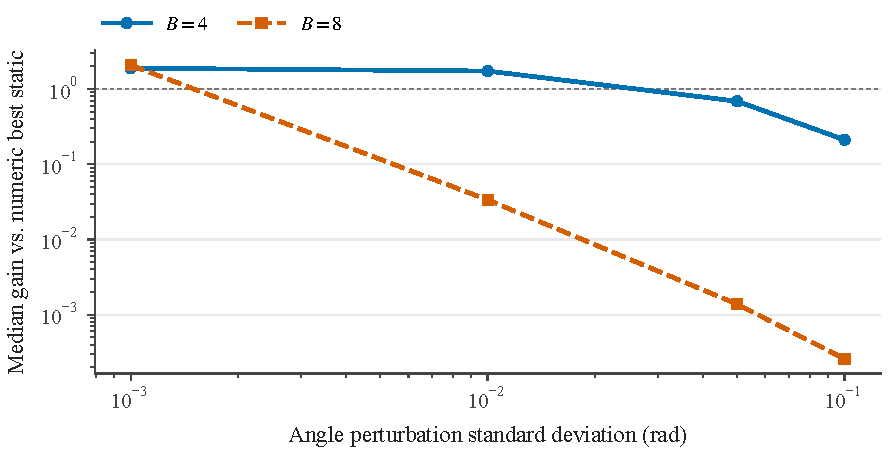
\includegraphics[width=.92\linewidth]{figures/geometry_robustness.pdf}
\caption{Sensitivity of the nominal preparation schedule. There are 24 independent perturbations per point. The long-budget gain is much more sensitive to small rotations. A value below one means preparation is worse.}\label{fig:robust}
\end{figure}

\subsection{Spectral and capacity experiments}
Each block is the $45^\circ$ family, with source scales $\lambda_j=j^{-1}$ and normalized initial masses proportional to $j^{-1-\beta}$ for $\beta\in\{0.5,1,2\}$. Ridge is 0 or 0.1 within the base block, and is scaled together with the block. There are 2,048 trained blocks and budgets 4, 16, 64, 256. The entire tail beyond the trained blocks is included using the Hurwitz zeta function. The balanced mixture is analytically best among all static weights because it is best in each block separately.

A two-phase candidate is parameterized by $(p_1,p_2,f)\in[0,1]^3$, with durations $fB$ and $(1-f)B$. A local L-BFGS-B search uses six starting points: $(0.5,0.5,0.5)$, $(1,0,0.15)$, $(1,0,0.5)$, $(0.9,0.1,0.3)$, $(0.8,0.1,0.7)$, and $(0.9,0.3,0.5)$. Its maximum iteration and function-call budgets are 80 and 500, with function tolerance $10^{-11}$ and gradient tolerance $10^{-10}$. The static candidate is always included. This procedure does not certify a global two-phase optimum. It only asks whether a small numerical search finds a substantial shared-schedule improvement.

The capacity experiment uses $(\alpha,\beta)=(1,1),(1,2),(2,1)$, 26 total-work budgets logarithmically spaced between $10^2$ and $10^7$, and a fixed list of capacities obtained by rounding 97 logarithmically spaced values between 2 and 32,768 and removing duplicates. For each capacity, $B=C/J$ and the balanced static risk is exact. Slopes fit the final ten budget points by least squares in log coordinates. Capacity selection is over this grid, whereas the theorem concerns all integer capacities; the slope check is not a global finite-budget capacity certificate.

\begin{figure}[t]
\centering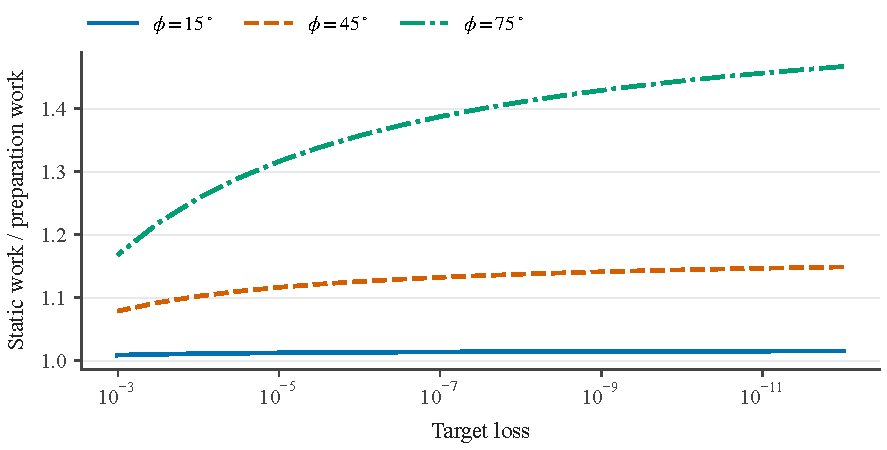
\includegraphics[width=.92\linewidth]{figures/work_savings.pdf}
\caption{Exact compute-to-target ratios for the known-direction construction. Even where the equal-work loss ratio diverges, the work ratio approaches the finite limit $1/a$ at zero ridge. The asymptotic regime is approached slowly for nearly orthogonal sources because preparation is expensive.}\label{fig:work}
\end{figure}

\subsection{Pilot and planning-cost experiment}
The known source angle is $45^\circ$ with no ridge. True unit residual directions are the bisector plus nine offsets equally spaced between $-0.06$ and $0.06$ radians. For each total budget $B\in\{4,8\}$, coordinate noise $\sigma\in\{0.05,0.2\}$, sample count per coordinate $n\in\{64,256,1024\}$, and query price $q\in\{10^{-4},10^{-3}\}$, we run 90 observations cycling over the nine true directions. We compare planning charges $h=0$ and $h=0.02$ using identical observation draws. There are 2,160 cases per charge, 4,320 rows total. The confidence level is $1-\delta=0.95$; the conservative Gaussian radius covers 2,158 cases for each charge.

The remaining training budget is exactly $B-2nq-h$. Both the $A$-then-$B$ and $B$-then-$A$ preparation schedules are evaluated at that remaining budget. The smaller risk upper bound chooses the candidate. The full-budget static lower envelope uses 2,048 cells at $B=4$ and 8,192 cells at $B=8$. On rejection, a static weight minimizing estimated-state risk over 512 cell centers is trained with the remaining budget. For descriptive gain and false-acceptance checks, a separate 1,025-point static grid with local refinement evaluates the true residual at the original budget. The certificate itself does not use this hidden reference value.

\begin{table}[h]
\centering\small
\caption{Pilot cost matters even when accepted decisions are correct. Medians use static risk divided by selected risk.}\label{tab:pilot}
\begin{tabular}{rrrrr}\toprule
Planning charge & Accepts / cases & False accepts & Accepted median & All-case median\\\midrule
0 & 25 / 2,160 & 0 & 1.447 & 0.417\\
0.02 & 23 / 2,160 & 0 & 1.400 & 0.403\\
\bottomrule\end{tabular}
\end{table}

The prices $q$ and $h$ are declared cost-model parameters. We do not infer them from processor clocks, nor claim that $h=0.02$ is the actual cost of every planner implementation. A real application must calibrate these prices and also decide whether to run the pilot. Neither a zero false-acceptance count nor a correct conditional theorem makes that initial purchase automatically beneficial.

\subsection{Finite-data linear training}
For each source, draw $x\sim N(0,G_i)$ and $y=x^\top\theta^*+\xi$, where $\theta^*=-u$ and $\xi\sim N(0,\sigma_y^2)$. Both source covariances include ridge $0.02$. Each source provides a cached dataset of $n\in\{128,1024\}$ samples. Source angles are 45 and 70 degrees; label standard deviation is 0 or 0.1; normalized budgets are 4 or 8. These are 16 settings, with 20 independent training/data seeds each.

SGD starts at zero, uses step size 0.025 and batch size 32, and draws with replacement from the cached source datasets. The static weight is implemented as the probability that each batch position uses source $A$. Within a seed, all methods share datasets, indices, and uniform mixture draws. The explicit preparation time is rounded to a step boundary. There are 11 static probabilities $0,0.1,\ldots,1$, both preparation orders, an exposure-matched static probability, and a greedy oracle choosing the source with larger current population quadratic decrease. Every trained run uses the same number of gradient examples at a fixed budget.

The principal comparator takes the minimum target risk over the 11 static weights separately for each realized seed. This is a stronger benchmark than selecting a weight on independent validation data, and its tuning cost is not charged. It is not a proposed deployable algorithm. This choice makes positive comparisons more demanding, but also means an average gain below one does not show that no practical schedule could help. All method-level risks, including the greedy and exposure-matched baselines, are retained in the raw CSV.

\begin{table}[h]
\centering\small
\caption{Preparation versus hindsight static grid in all 16 linear settings. Intervals are paired percentile bootstrap intervals for the median gain across 20 seeds.}\label{tab:linear}
\begin{tabular}{rrrrrr}\toprule
Angle & Noise & Samples/source & Budget & Median [95\% interval] & Wins\\\midrule
45 & 0 & 128 & 4 & 0.863 [0.662, 1.432] & 9/20 \\
45 & 0 & 128 & 8 & 0.104 [0.060, 0.286] & 4/20 \\
45 & 0 & 1024 & 4 & 1.513 [1.268, 1.637] & 18/20 \\
45 & 0 & 1024 & 8 & 0.192 [0.059, 0.334] & 2/20 \\
45 & 0.1 & 128 & 4 & 0.913 [0.518, 1.141] & 8/20 \\
45 & 0.1 & 128 & 8 & 0.130 [0.084, 0.319] & 3/20 \\
45 & 0.1 & 1024 & 4 & 1.569 [1.248, 1.813] & 17/20 \\
45 & 0.1 & 1024 & 8 & 0.294 [0.123, 0.681] & 4/20 \\
70 & 0 & 128 & 4 & 1.665 [1.290, 2.018] & 19/20 \\
70 & 0 & 128 & 8 & 0.095 [0.020, 0.286] & 3/20 \\
70 & 0 & 1024 & 4 & 2.582 [2.081, 2.750] & 20/20 \\
70 & 0 & 1024 & 8 & 0.519 [0.104, 2.176] & 7/20 \\
70 & 0.1 & 128 & 4 & 1.841 [1.297, 2.232] & 17/20 \\
70 & 0.1 & 128 & 8 & 0.208 [0.169, 0.508] & 3/20 \\
70 & 0.1 & 1024 & 4 & 2.285 [1.955, 2.443] & 20/20 \\
70 & 0.1 & 1024 & 8 & 0.388 [0.199, 0.998] & 5/20 \\
\bottomrule\end{tabular}
\end{table}

\subsection{Fully trained nonlinear stress test}
The source distributions have angle $45^\circ$ and ridge $0.05$. Each cached source has 512 examples; the teacher remains linear. A two-layer network
\[
 f(x)=v^\top\tanh(Wx+b)+c
\]
has input dimension two and width 16. Hidden weights are initialized independently from $N(0,0.5^2)$, output weights and biases are zero, and all parameters are updated by SGD. The learning rate is 0.02, batch size is 32, and training lasts 200 or 800 steps, with label standard deviation 0 or 0.1. The test set contains 4,096 independent standard-Gaussian inputs and noiseless teacher labels, fixed across methods.

For this stress test, the linear-model switch \emph{fraction} is transferred using reference budgets 4 and 8 for the 200- and 800-step settings respectively. In particular, 800 neural steps times learning rate 0.02 is not claimed to equal reference budget 8 or to implement the quadratic flow. The budget for neural comparisons is the actual number of steps and processed examples. This is a heuristic schedule-transfer experiment, not a test that a nonlinear Hessian obeys the theorem. Five static probabilities, both preparation orders, and the exposure-matched static probability use the same initialization and stochastic draws within each seed. There are 12 independent seeds per setting. A finite-difference unit test independently checks the manual backpropagation equations.

\begin{table}[h]
\centering\small
\caption{All nonlinear conditions. No condition has a median gain above one.}\label{tab:nonlinear}
\begin{tabular}{rrrr}\toprule
Label noise & Training steps & Median gain [95\% interval] & Wins / 12\\\midrule
0 & 200 & 0.925 [0.677, 1.058] & 5/12 \\
0 & 800 & 0.895 [0.784, 0.997] & 3/12 \\
0.1 & 200 & 0.901 [0.824, 0.981] & 2/12 \\
0.1 & 800 & 0.863 [0.782, 0.928] & 1/12 \\
\bottomrule\end{tabular}
\end{table}

\begin{figure}[t]
\centering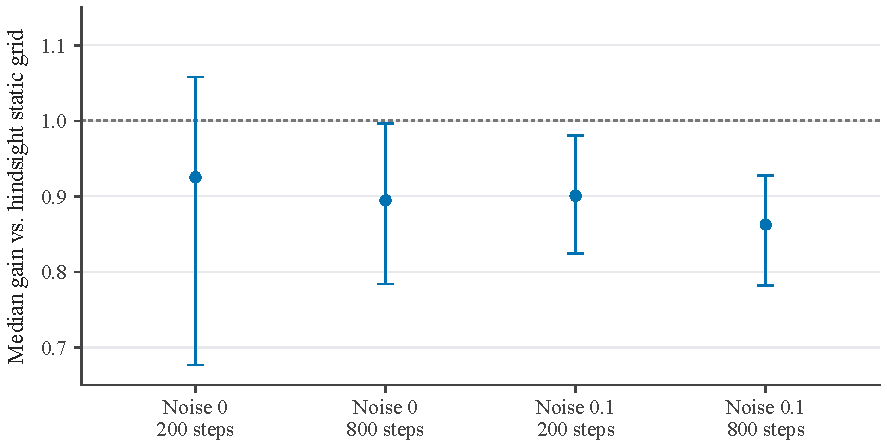
\includegraphics[width=.92\linewidth]{figures/nonlinear_gain.pdf}
\caption{The negative nonlinear stress test. Both layers learn, so this is not a fixed random-feature model. Error bars show unadjusted paired 95\% bootstrap intervals for median gain versus a per-seed hindsight static grid.}\label{fig:nonlinear}
\end{figure}

\subsection{Statistics, reproducibility, and reporting scope}
The linear and nonlinear summary intervals use 4,000 percentile-bootstrap resamples of paired gain ratios, with seed 91021. Independent units are data/training seeds, not individual examples or optimization steps. The intervals are descriptive and are not adjusted for comparisons across settings. They do not quantify uncertainty about transfer to different tasks. The exact-matrix and capacity curves are deterministic and do not need error bars. Pilot simulations are controlled scenarios, not trials sampled from a real deployment population.

The release records Python and package versions per suite, raw scientific CSVs, deterministic summary scripts, separate matplotlib figures, and an artifact integrity manifest. Scientific CSV reproducibility is checked separately from runtime metadata. Random generators use NumPy's default generator with explicit seeds. Tests include analytic family identities, Golden--Thompson comparisons, the conditioning bound, commuting controls, the two-phase lower bound, state-ball envelopes, Duhamel perturbations, independent high-precision matrix exponentials, volume bounds, spectral implementation equivalence, and neural finite differences. Passing these tests is evidence of implementation consistency, not a substitute for an independent mathematical review.


\end{document}
